% =====================================================================
%  Eigenständiges Vorschau-Dokument für die EBM-Anleitung.
%  Dient nur zum Kompilieren/Ansehen der Anleitung als PDF.
%  Der eigentliche Inhalt steckt in anleitung.tex und wird per \input
%  eingebunden -- genau so, wie es im Hauptdokument des Kollegen geschieht.
%
%  Kompilieren:  pdflatex anleitung_standalone.tex
% =====================================================================
\documentclass[11pt,a4paper]{article}

\usepackage[utf8]{inputenc}
\usepackage[T1]{fontenc}
\usepackage[ngerman]{babel}
\usepackage{graphicx}
\usepackage{booktabs}
\usepackage{float}
\usepackage{amssymb}   % für die Symbole der App-Buttons (Play/Stopp)
\usepackage[a4paper,margin=2.5cm]{geometry}
\usepackage[hidelinks]{hyperref}

% Grafikpfad: Screenshots liegen relativ zu dieser Datei.
\graphicspath{{./}{screenshots/}}

\title{EBM Strategy Converter\\\large Kurzanleitung zur Bedienung}
\author{}
\date{}

\begin{document}
\maketitle

% =====================================================================
%  Kurzanleitung: EBM Strategy Converter – Desktop Edition
%  ---------------------------------------------------------------------
%  Zum Einbinden in ein bestehendes LaTeX-Dokument gedacht.
%
%  Einbinden per:   % =====================================================================
%  Kurzanleitung: EBM Strategy Converter – Desktop Edition
%  ---------------------------------------------------------------------
%  Zum Einbinden in ein bestehendes LaTeX-Dokument gedacht.
%
%  Einbinden per:   % =====================================================================
%  Kurzanleitung: EBM Strategy Converter – Desktop Edition
%  ---------------------------------------------------------------------
%  Zum Einbinden in ein bestehendes LaTeX-Dokument gedacht.
%
%  Einbinden per:   \input{anleitung.tex}
%
%  Benötigte Pakete (im Hauptdokument in der Präambel):
%     \usepackage{graphicx}
%     \usepackage{booktabs}
%     \usepackage{float}
%     \usepackage{amssymb}               % für ▶/■-Symbole (sonst greift unten ein Fallback)
%     \usepackage[hidelinks]{hyperref}   % optional
%
%  Die Screenshots liegen im Unterordner  screenshots/ .
%  Ggf. den Grafikpfad im Hauptdokument setzen:
%     \graphicspath{{screenshots/}}
%  oder in den \includegraphics-Befehlen den Pfad anpassen.
% =====================================================================

% Fallback: Falls amssymb nicht geladen ist, einfache Ersatzsymbole
% definieren, damit das Dokument trotzdem kompiliert (\triangleright und
% \bullet stammen aus dem LaTeX-Kern und sind immer verfügbar).
\providecommand{\blacktriangleright}{\ensuremath{\triangleright}}
\providecommand{\blacksquare}{\ensuremath{\bullet}}

\section{Bedienung der Software: EBM Strategy Converter}
\label{sec:ebm-anleitung}

Der \emph{EBM Strategy Converter} ist ein Desktop-Werkzeug, das die
Belichtungsreihenfolge (Scan-Strategie) für den Elektronenstrahl-Schmelzprozess
des Arcam~S12 Pro-Beam neu anordnet. Die Software liest ein Baujob-ZIP-Archiv
mit \texttt{.B99}-Punktwolkendateien ein, sortiert die Schmelzpunkte der
Infill-Schichten nach einer frei wählbaren Strategie um und schreibt ein
druckfertiges ZIP zurück. Dabei wird \textbf{keine einzige Koordinate
verändert} -- es ändert sich ausschließlich die \emph{Reihenfolge}, in der die
Punkte belichtet werden.

Die folgende Anleitung beschreibt den Arbeitsablauf in vier Schritten:
ZIP laden $\rightarrow$ Strategie wählen $\rightarrow$ Vorschau prüfen
$\rightarrow$ ZIP exportieren.

% ---------------------------------------------------------------------
\subsection{Überblick über die Oberfläche}
\label{subsec:ebm-overview}

Nach dem Start zeigt das Programm links eine interaktive 3D-Vorschau und rechts
ein Bedien-Panel mit fünf Bereichen: \emph{Projekt}, \emph{Vorschau},
\emph{Strategie}, \emph{Simulation} und \emph{Export}
(Abbildung~\ref{fig:ebm-start}). Die 3D-Ansicht lässt sich mit der Maus drehen
(linke Maustaste) und zoomen (Mausrad).

\begin{figure}[H]
  \centering
  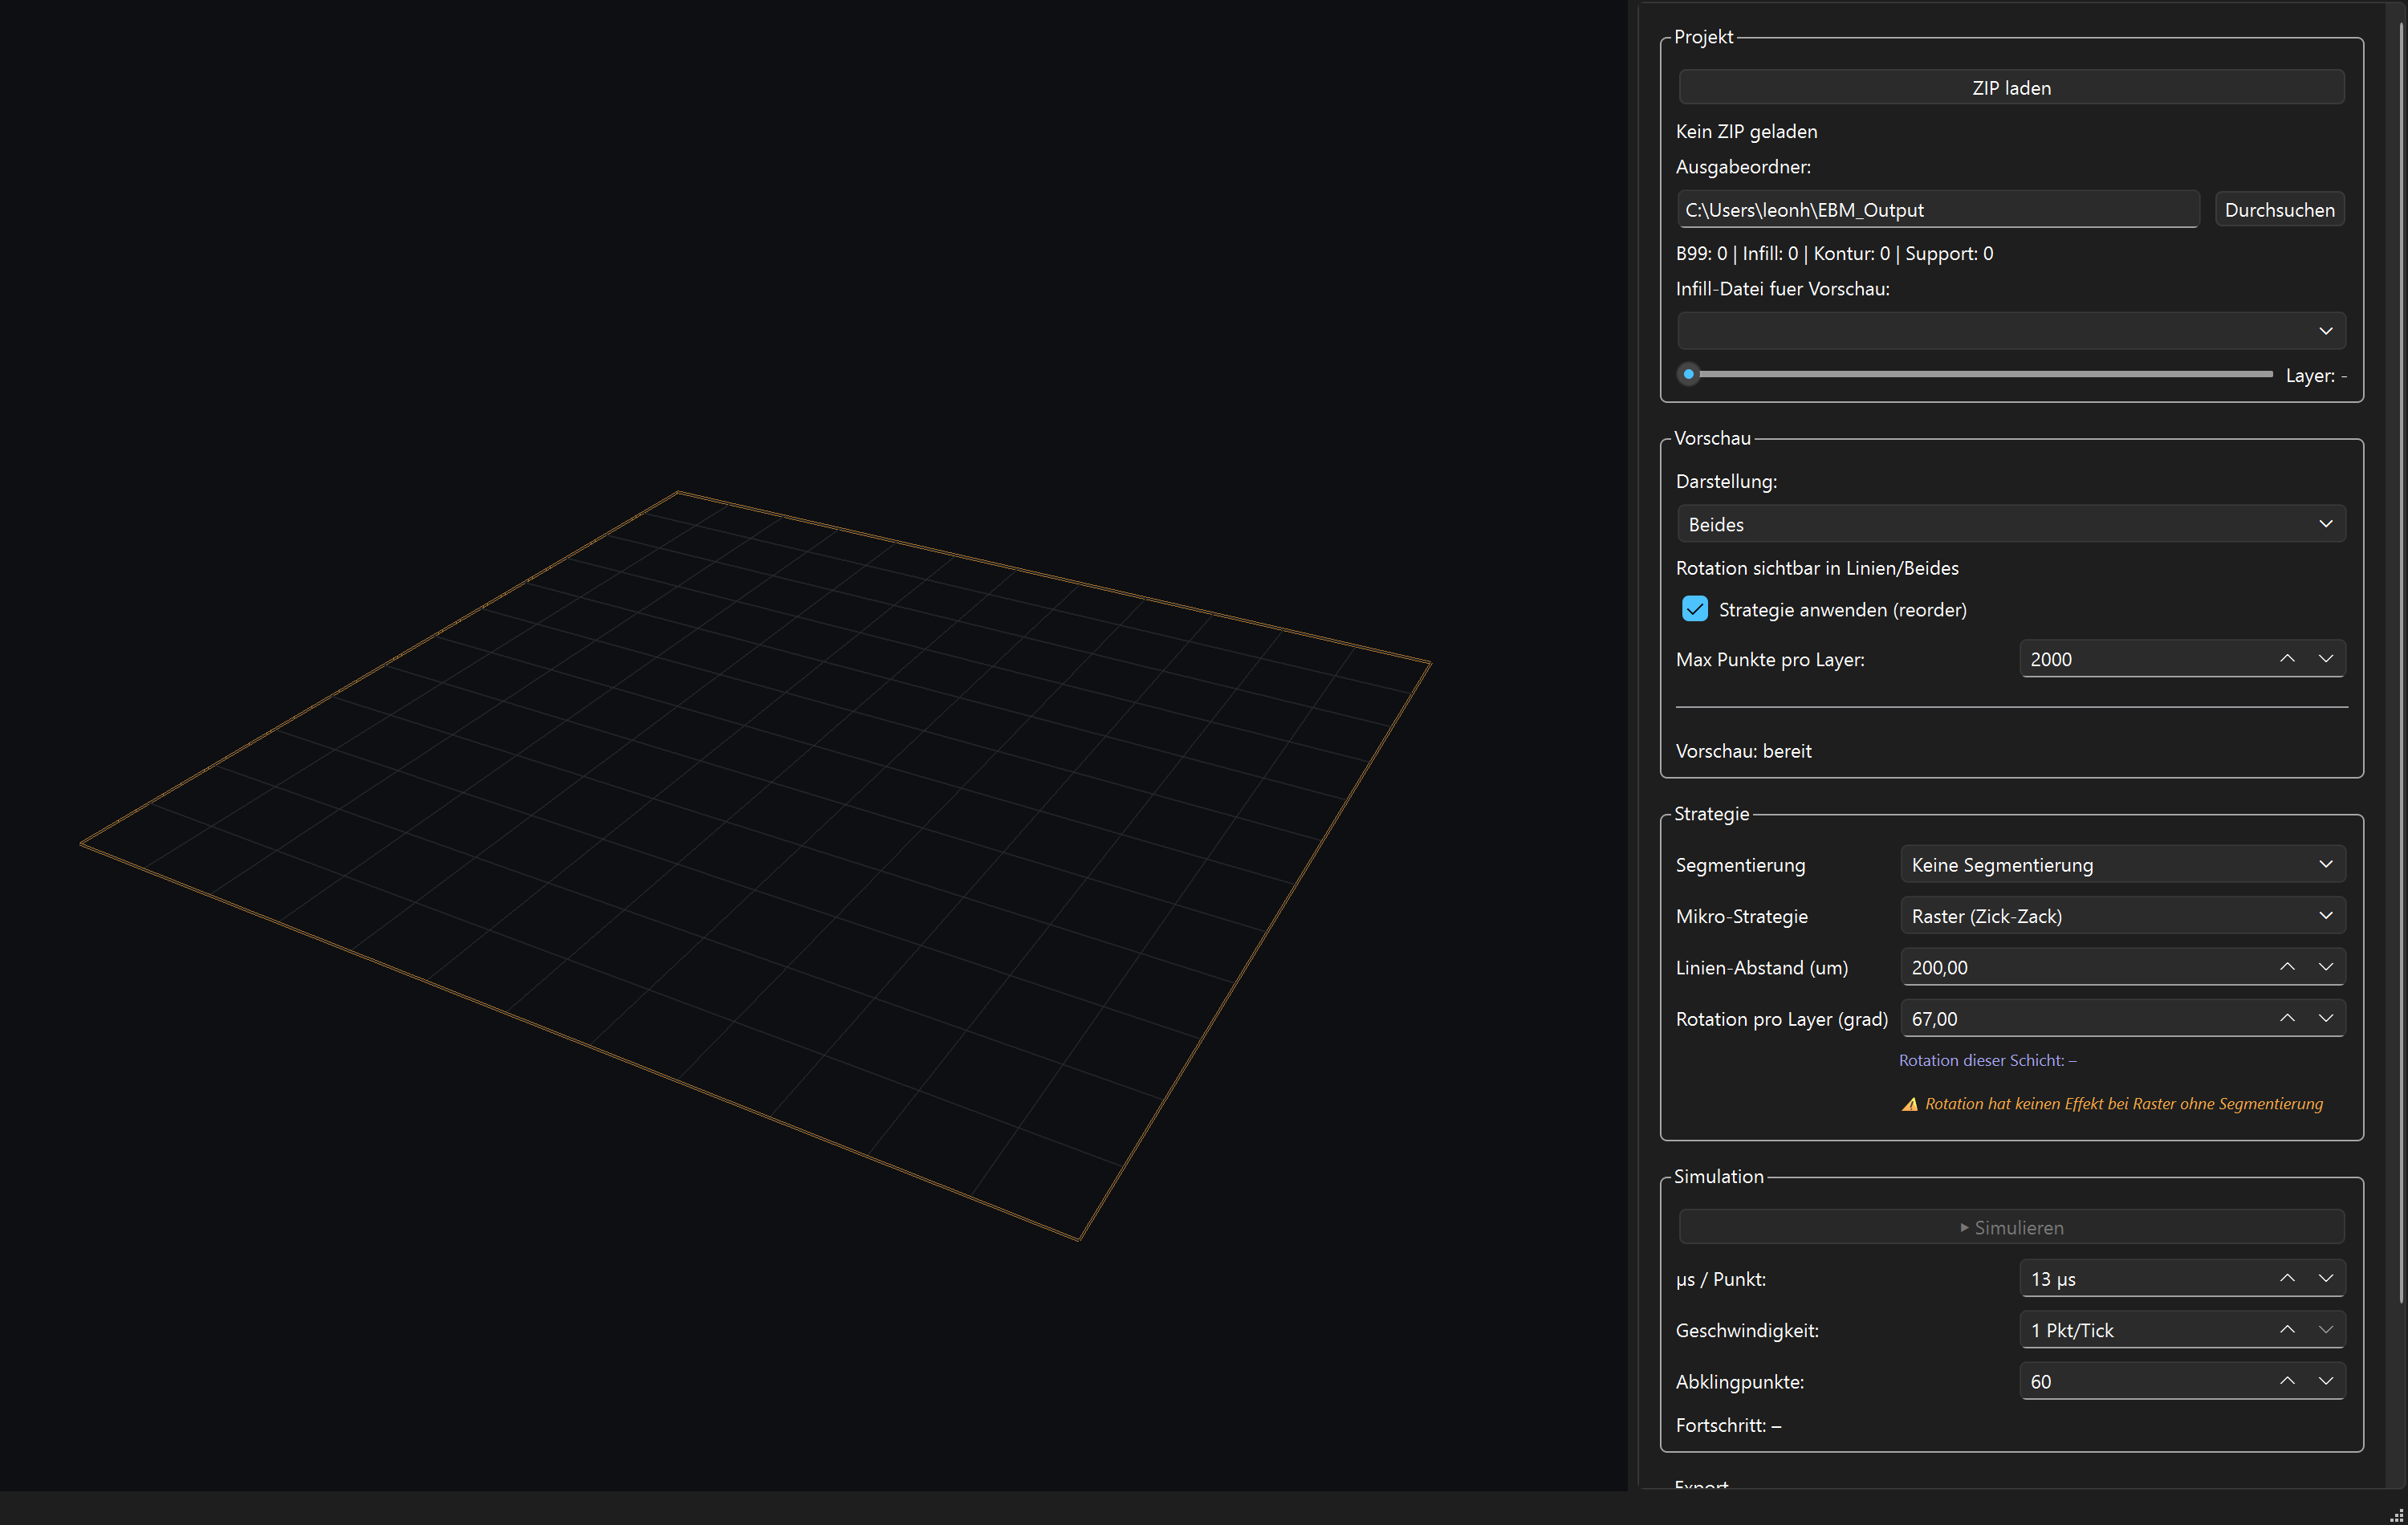
\includegraphics[width=\linewidth]{screenshots/01_startfenster.png}
  \caption{Startfenster nach dem Programmstart. Links die noch leere
           3D-Vorschau (Bauplattform 120\,$\times$\,120\,mm), rechts das
           Bedien-Panel.}
  \label{fig:ebm-start}
\end{figure}

% ---------------------------------------------------------------------
\subsection{Schritt 1 -- Baujob-ZIP laden}
\label{subsec:ebm-load}

Über die Schaltfläche \textbf{ZIP laden} im Bereich \emph{Projekt} wird ein
Baujob-Archiv geöffnet, das einen Ordner \texttt{Figure Files/} mit den
\texttt{.B99}-Dateien enthält (so, wie es die Arcam-Software exportiert). Im
Beispiel wird die Datei \texttt{20260408\_5Cubes\_0\_Rotation.zip}
geladen -- ein Baujob mit fünf Würfeln.

Nach dem Laden klassifiziert die Software alle Dateien automatisch und zeigt
eine Statistik an, z.\,B.\ \texttt{B99: 1466 | Infill: 745 | Kontur: 595 |
Support: 126}. Anschließend erscheint sofort eine 3D-Vorschau der ersten
Infill-Schicht (Abbildung~\ref{fig:ebm-loaded}).

\begin{itemize}
  \item \textbf{Ausgabeordner:} Zielordner für das exportierte ZIP
        (Standard: \texttt{\textasciitilde/EBM\_Output}).
  \item Das Auswahlfeld \textbf{Infill-Datei für Vorschau} und der
        \textbf{Layer-Schieberegler} wählen die anzuzeigende Schicht.
\end{itemize}

\begin{figure}[H]
  \centering
  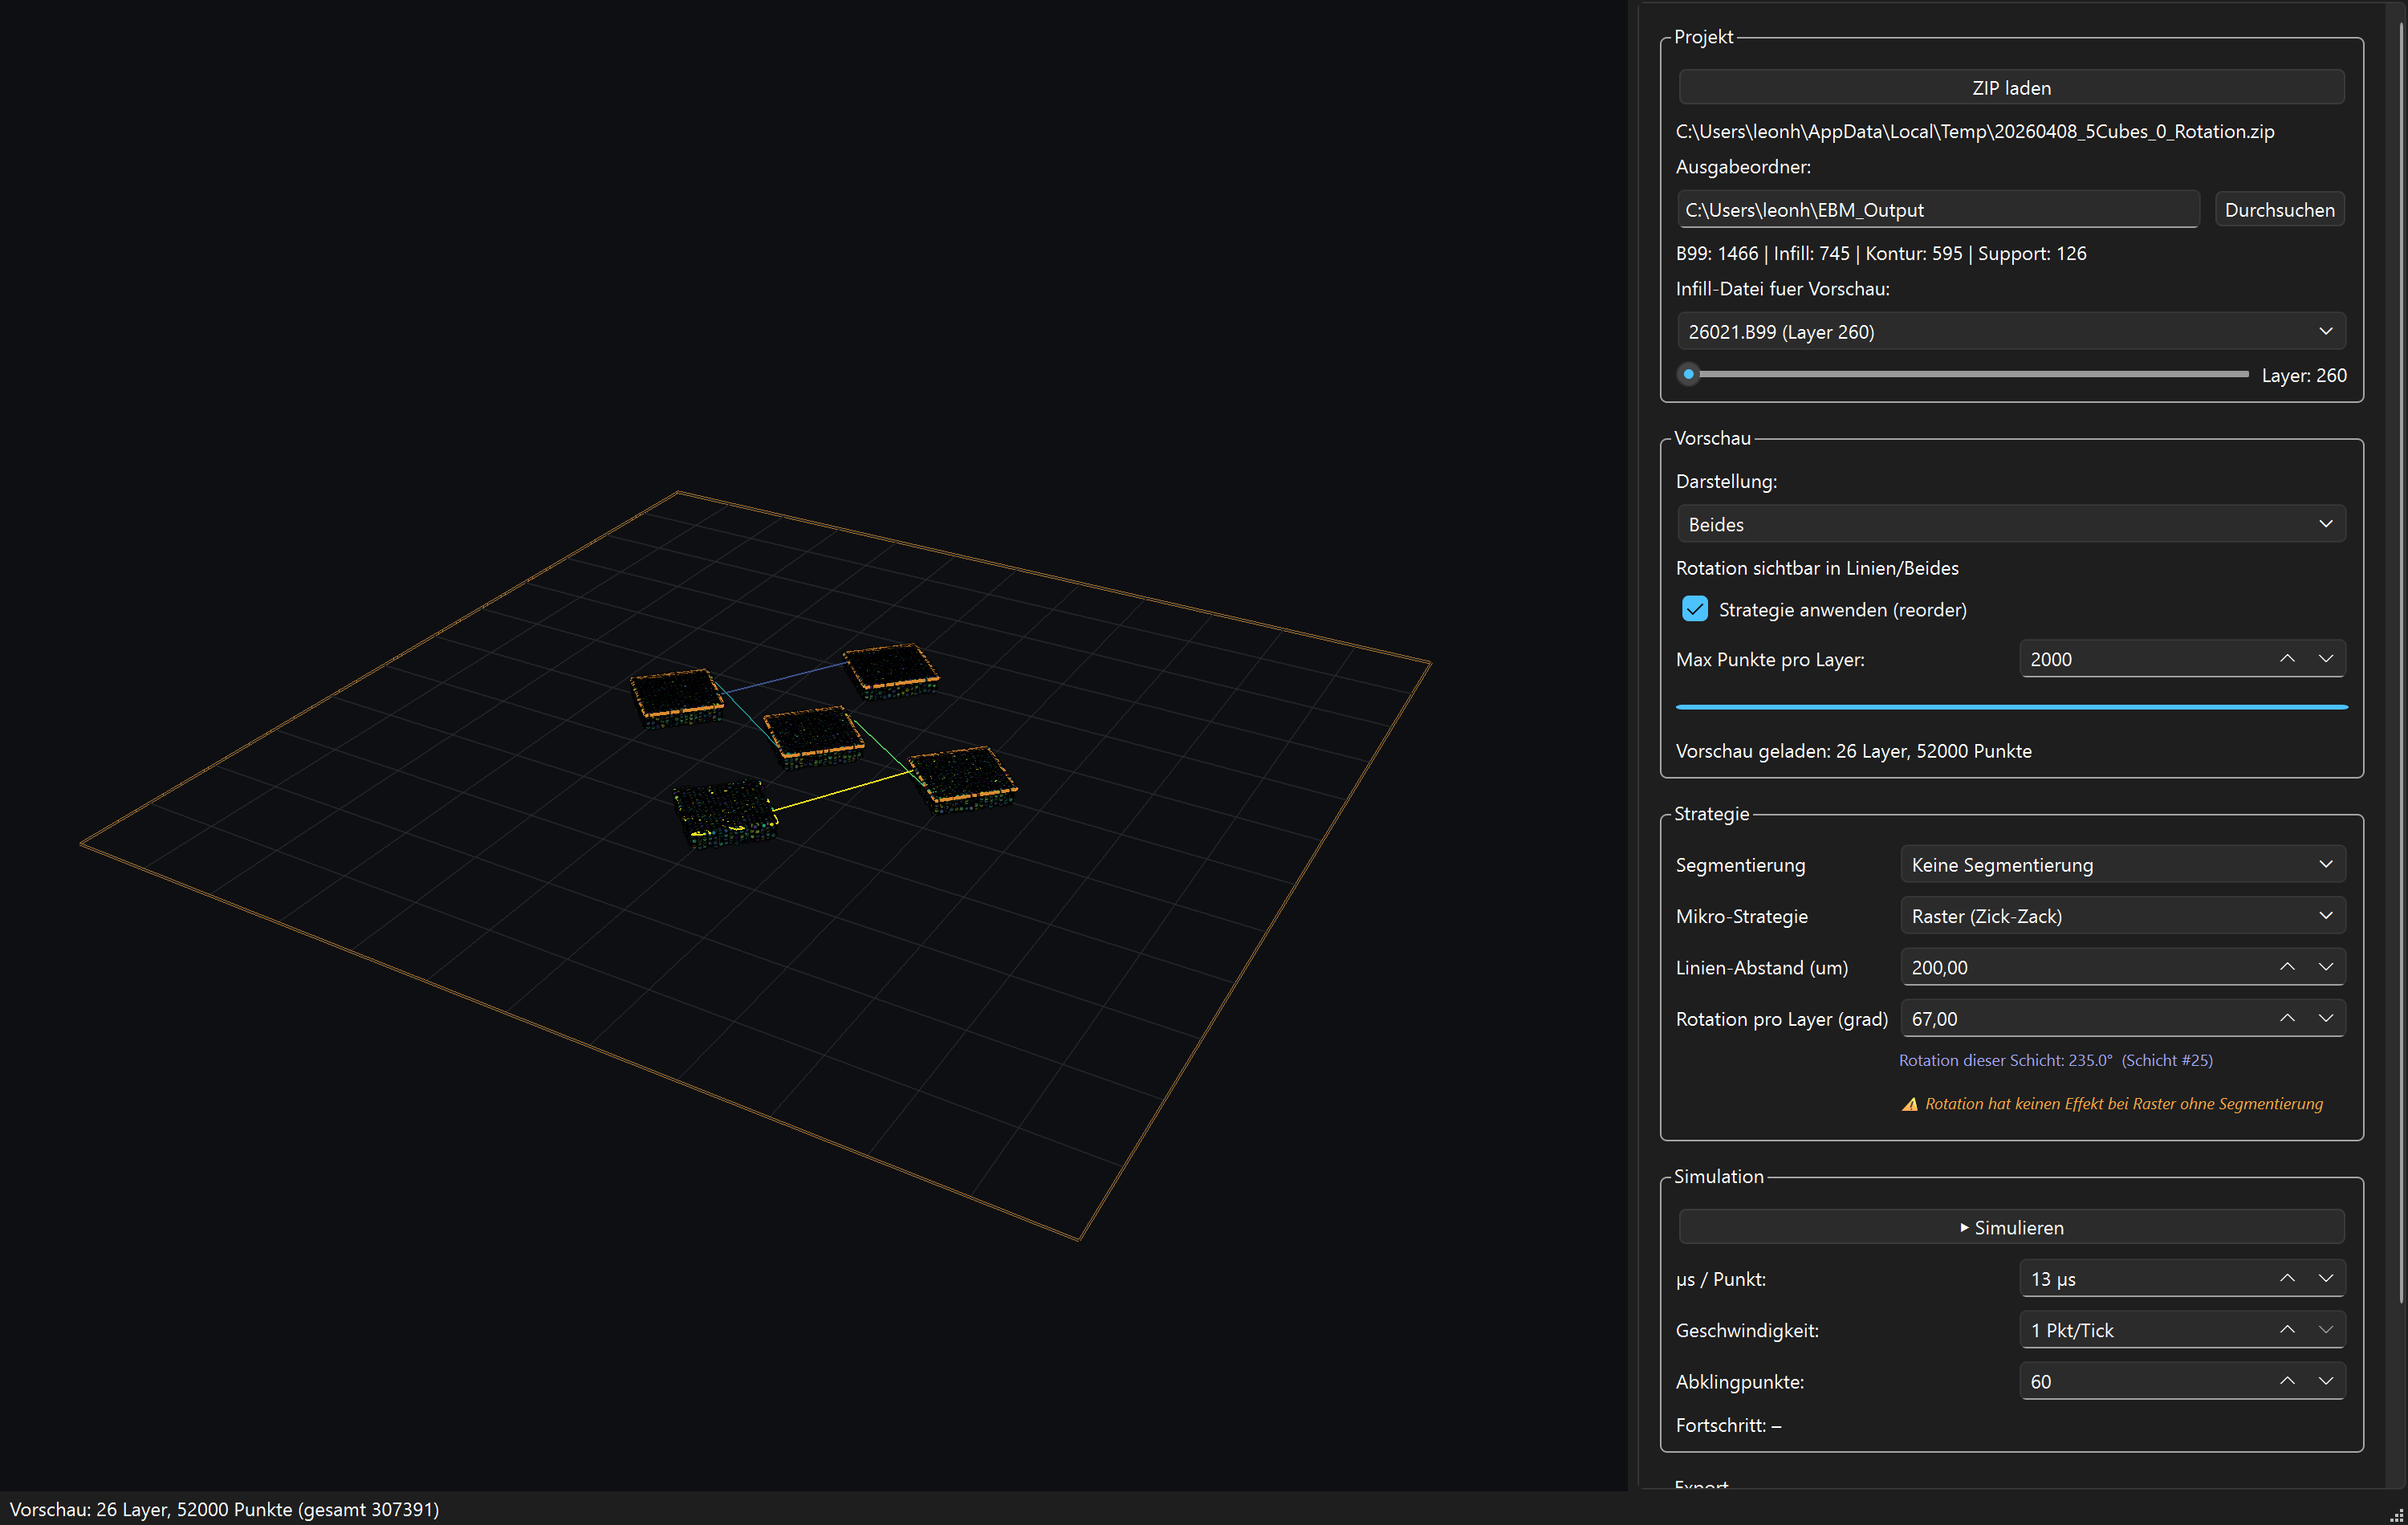
\includegraphics[width=\linewidth]{screenshots/02_projekt_geladen.png}
  \caption{Geladener Baujob. Die fünf Würfel sind als orange Konturen
           erkennbar, die farbigen Punkte zeigen die Infill-Belichtung der
           gewählten Schicht. Oben rechts die Datei-Statistik.}
  \label{fig:ebm-loaded}
\end{figure}

% ---------------------------------------------------------------------
\subsection{Schritt 2 -- Strategie konfigurieren}
\label{subsec:ebm-strategy}

Die Scan-Strategie besteht aus zwei unabhängigen Stufen, die im Bereich
\emph{Strategie} eingestellt werden (Abbildung~\ref{fig:ebm-panel}):

\paragraph{Stufe 1 -- Segmentierung (Makro).}
Legt fest, wie die Schicht grob in Bereiche aufgeteilt wird.

\begin{table}[H]
  \centering
  \begin{tabular}{@{}ll@{}}
    \toprule
    \textbf{Option} & \textbf{Beschreibung} \\
    \midrule
    Keine Segmentierung      & Alle Punkte als ein Block \\
    Schachbrett (Island)     & Quadratische Felder, abwechselnd belichtet \\
    Streifen (Stripe)        & Parallele Bänder \\
    Hexagonal                & Versetztes Waben-Gitter \\
    Spiralzonen              & Konzentrische Ringe um den Schwerpunkt \\
    \bottomrule
  \end{tabular}
  \caption{Verfügbare Segmentierungsarten (Stufe~1).}
  \label{tab:ebm-seg}
\end{table}

\paragraph{Stufe 2 -- Mikro-Strategie.}
Legt fest, in welcher Reihenfolge die Punkte \emph{innerhalb} eines Segments
belichtet werden -- z.\,B.\ \emph{Raster (Zick-Zack)},
\emph{Hilbert-Kurve}, \emph{Spiral} oder \emph{Ghost Beam}. Je nach Auswahl
blendet die Oberfläche die passenden Zusatzparameter ein bzw.\ aus.

\paragraph{Rotation pro Layer.}
Der Wert \emph{Rotation pro Layer (Grad)} dreht das Muster von Schicht zu
Schicht weiter: Schicht~$N$ wird um $N \times \mathrm{Winkel}$ (modulo
$360^\circ$) gedreht. Die Oberfläche zeigt darunter die effektive Rotation der
aktuell gewählten Schicht an (z.\,B.\ \texttt{Rotation dieser Schicht: 153{,}0$^\circ$}).

\begin{quote}
  \footnotesize\itshape
  Hinweis: Bei der Mikro-Strategie \emph{Raster} ohne Segmentierung hat die
  Rotation keinen Effekt -- die Software weist mit einem orangefarbenen
  Warnhinweis darauf hin.
\end{quote}

\begin{figure}[H]
  \centering
  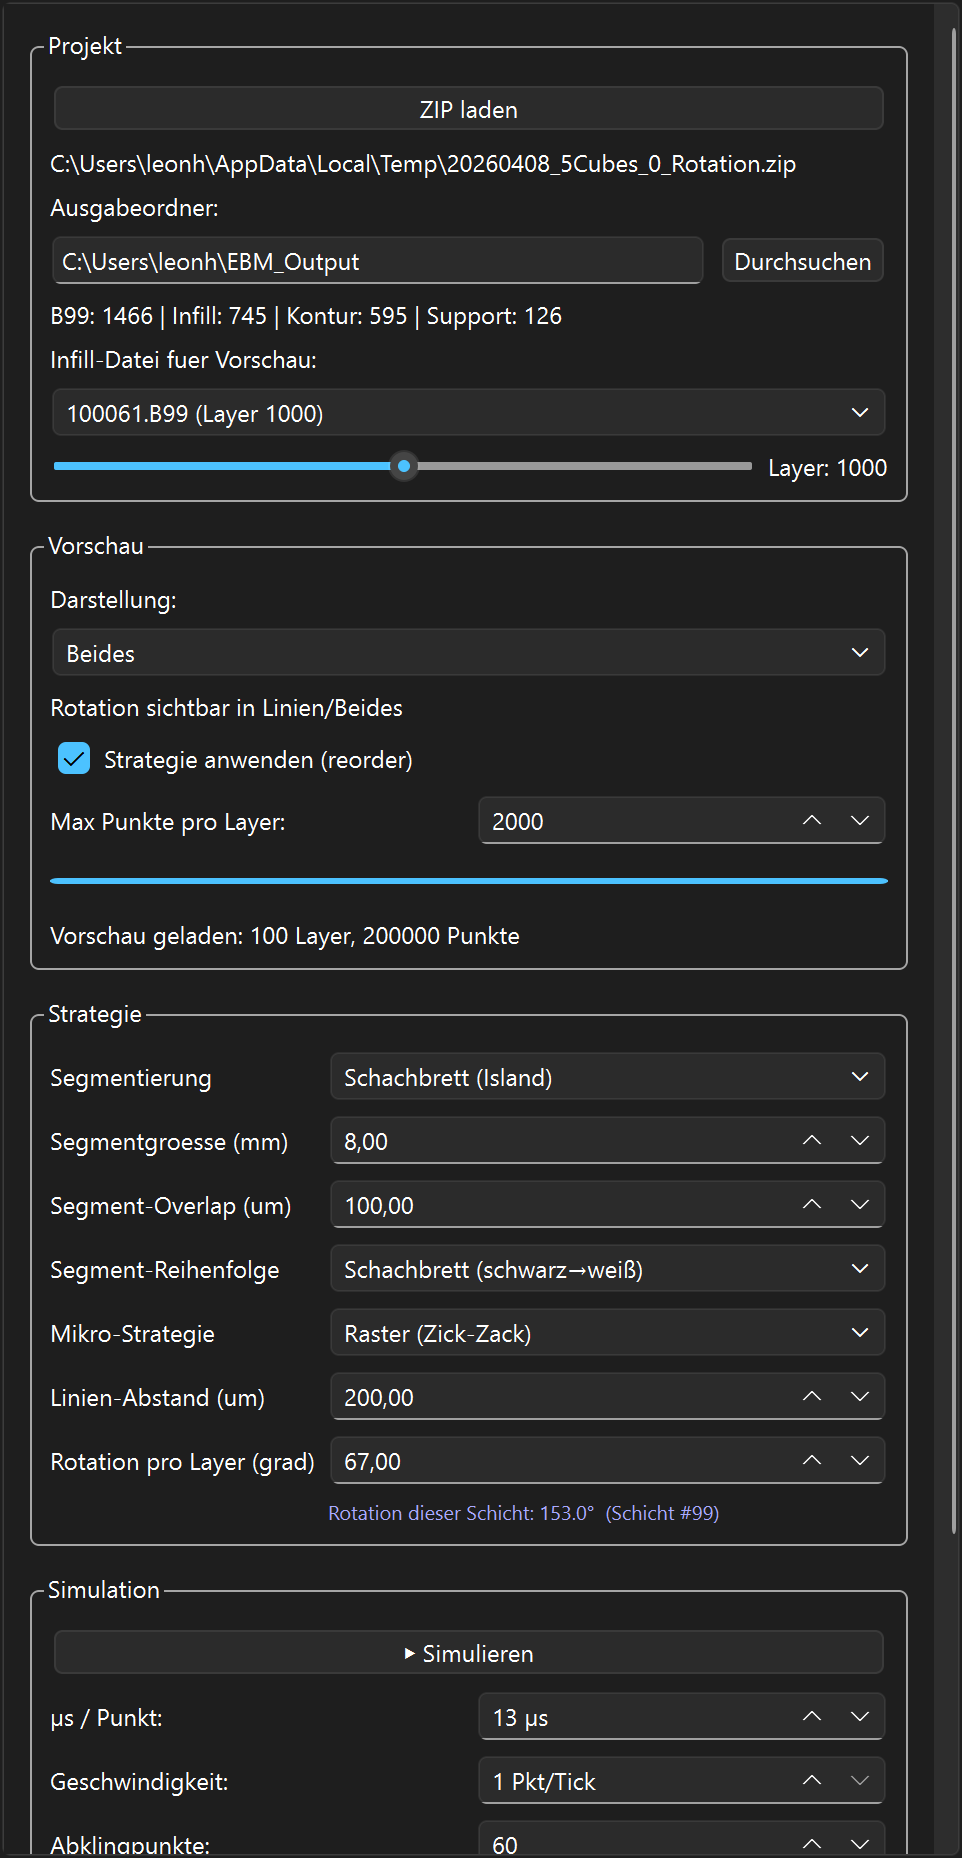
\includegraphics[height=0.82\textheight]{screenshots/04_bedienpanel.png}
  \caption{Das Bedien-Panel im Detail mit konfigurierter
           Schachbrett-Segmentierung und Raster-Mikrostrategie. Unter dem
           Rotationsfeld wird die effektive Rotation der aktuellen Schicht
           angezeigt.}
  \label{fig:ebm-panel}
\end{figure}

% ---------------------------------------------------------------------
\subsection{Schritt 3 -- Vorschau und Simulation prüfen}
\label{subsec:ebm-preview}

Im Bereich \emph{Vorschau} steuert das Feld \textbf{Darstellung} die Ansicht:
\emph{Punkte} zeigt nur die Schmelzpunkte, \emph{Linien} den Scan-Pfad und
\emph{Beides} die Kombination. Mit dem Schieberegler \emph{Layer} lässt sich
durch die Schichten blättern; jede Änderung an der Strategie aktualisiert die
Vorschau automatisch. Abbildung~\ref{fig:ebm-strategy} zeigt die
Schachbrett-Strategie über mehrere übereinanderliegende Schichten, wodurch die
schichtweise Rotation sichtbar wird.

\begin{figure}[H]
  \centering
  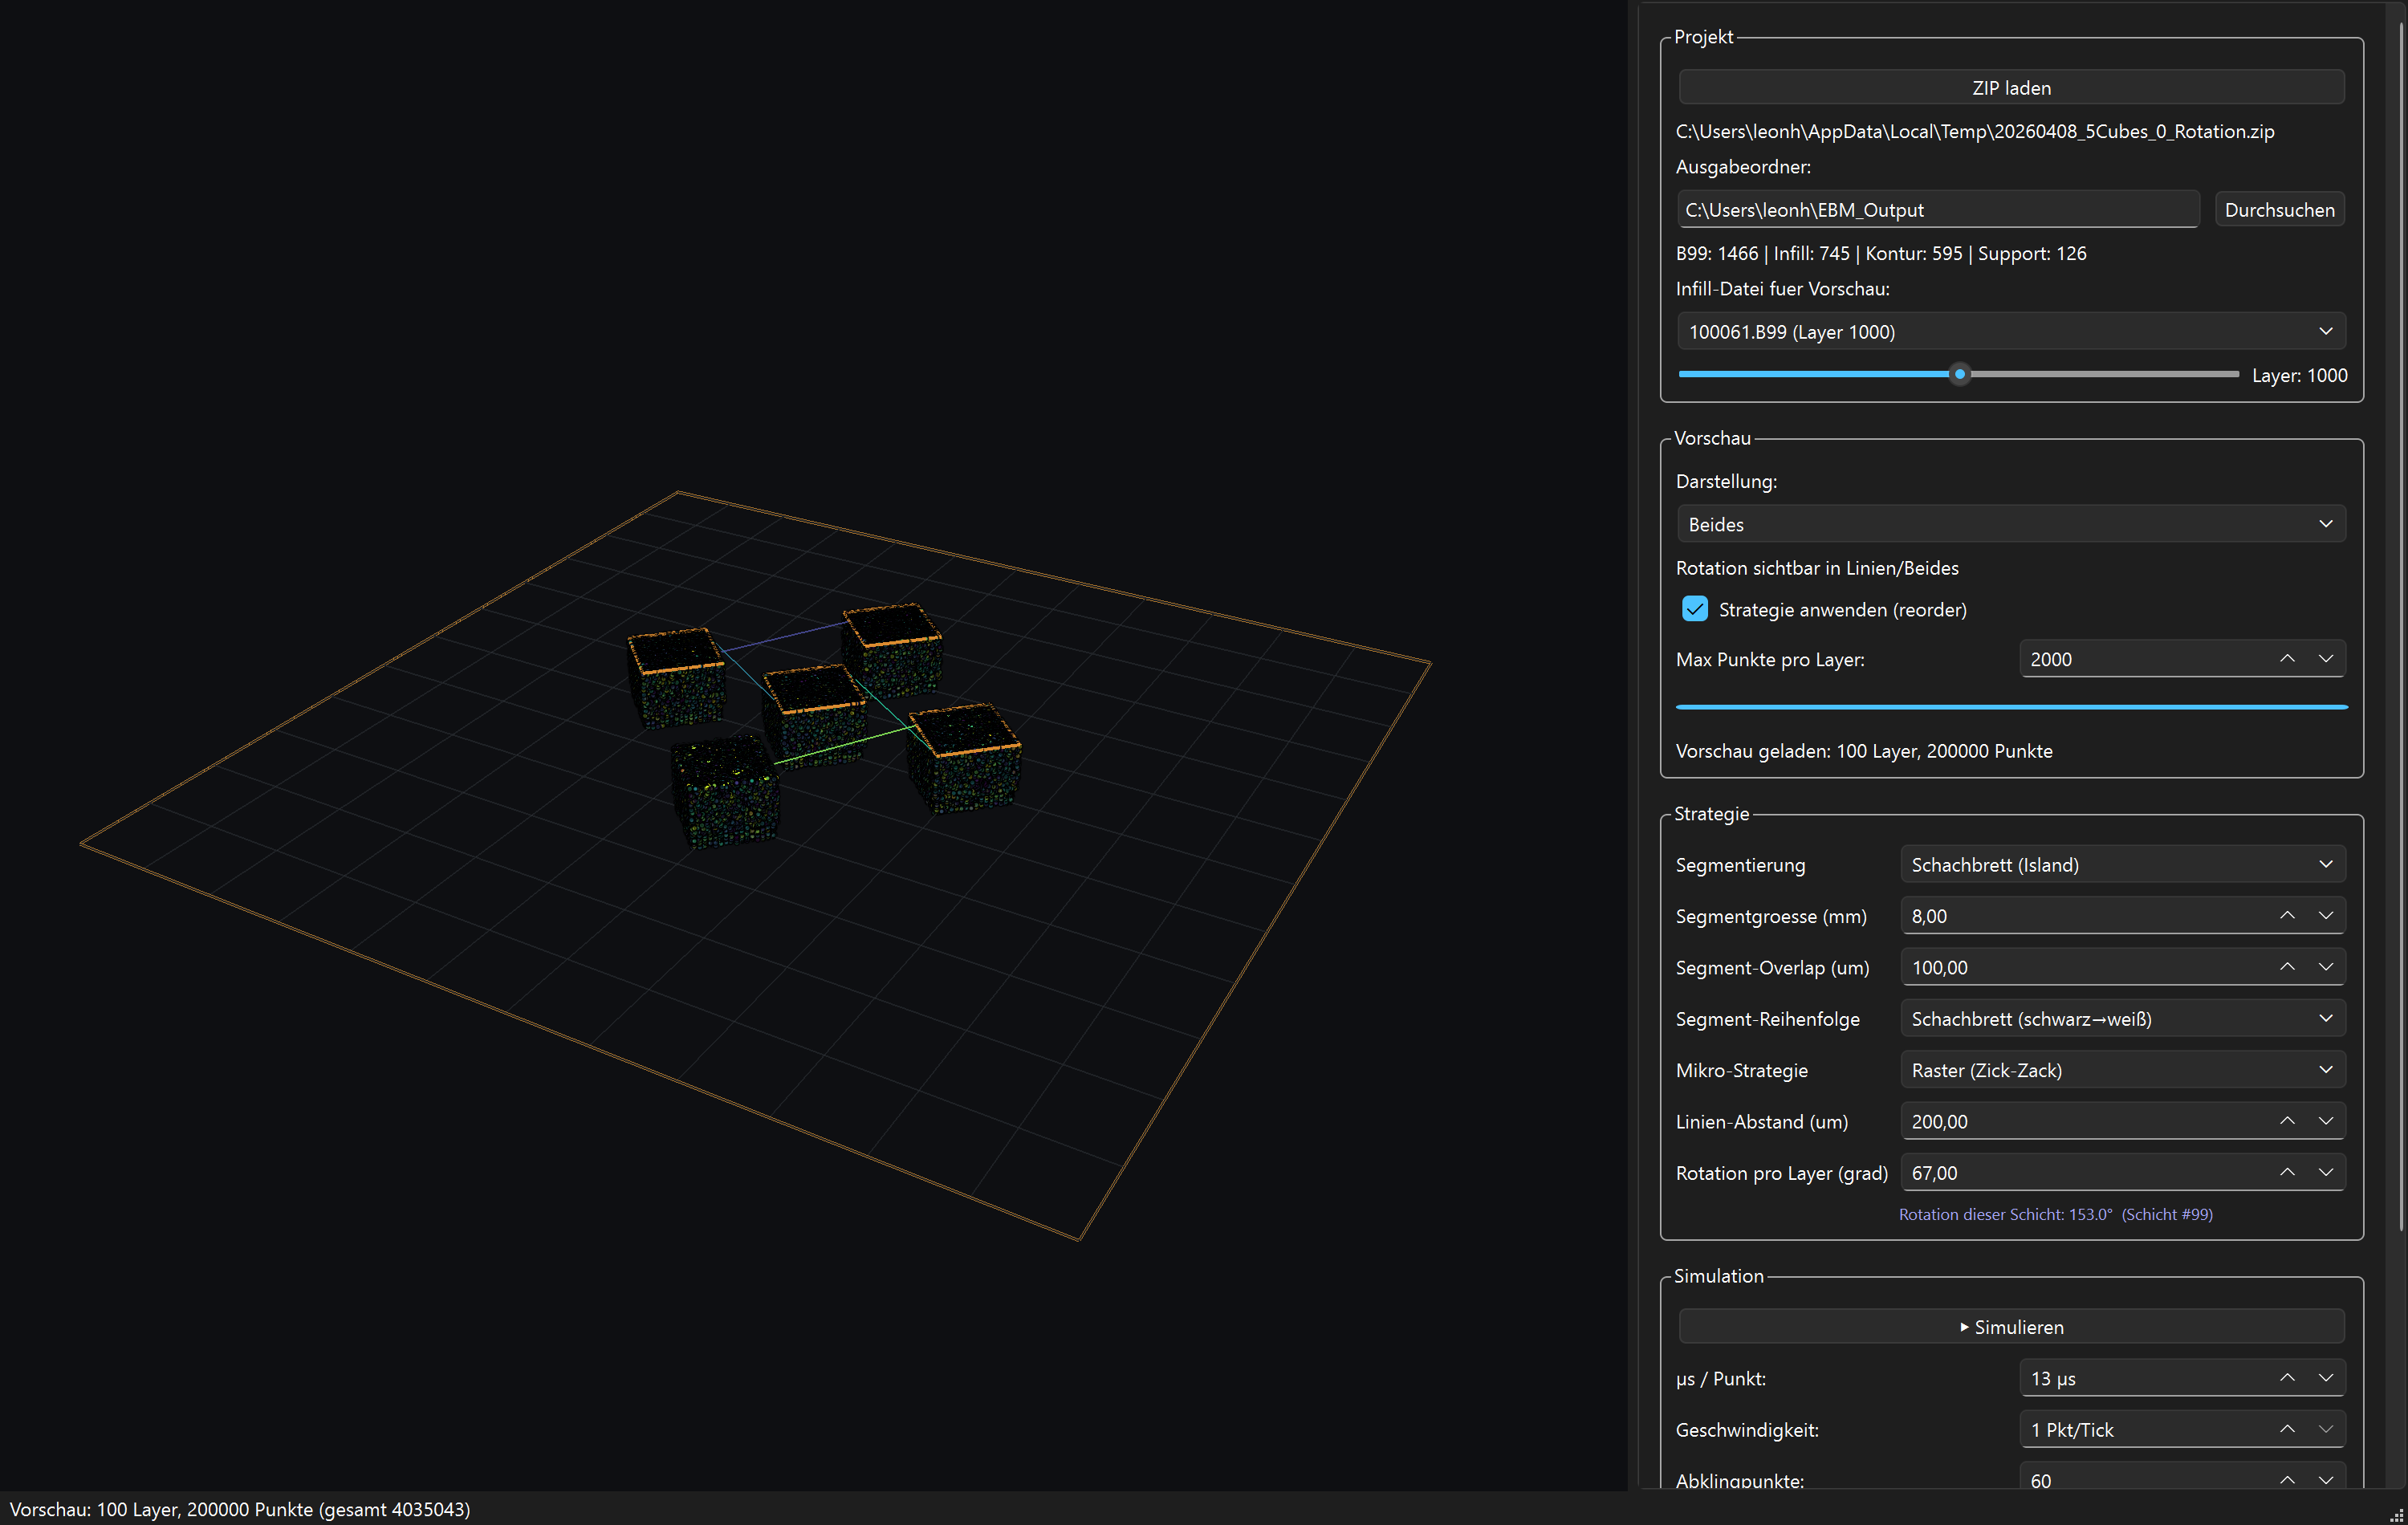
\includegraphics[width=\linewidth]{screenshots/03_strategie_vorschau.png}
  \caption{3D-Vorschau mit aktiver Schachbrett-Segmentierung und
           schichtweiser Rotation. Die grünen Linien zeigen den Scan-Pfad der
           aktuell gewählten Schicht.}
  \label{fig:ebm-strategy}
\end{figure}

\paragraph{Simulation.}
Über \textbf{$\blacktriangleright$~Simulieren} im Bereich \emph{Simulation}
wird die Belichtung der gewählten Schicht Punkt für Punkt animiert. Der gerade
belichtete Punkt leuchtet hell auf, bereits belichtete Punkte klingen langsam
ab -- so wird die Reihenfolge der Strategie unmittelbar nachvollziehbar
(Abbildung~\ref{fig:ebm-sim}). Die Parameter steuern das Tempo:

\begin{itemize}
  \item \textbf{$\mu$s / Punkt} -- realistische Haltezeit pro Punkt
        (typisch 13\,$\mu$s).
  \item \textbf{Geschwindigkeit (Pkt/Tick)} -- wie viele Punkte pro Animations-
        schritt gezeichnet werden; höhere Werte beschleunigen den Durchlauf.
  \item \textbf{Abklingpunkte} -- Länge der nachleuchtenden Spur.
\end{itemize}

\begin{figure}[H]
  \centering
  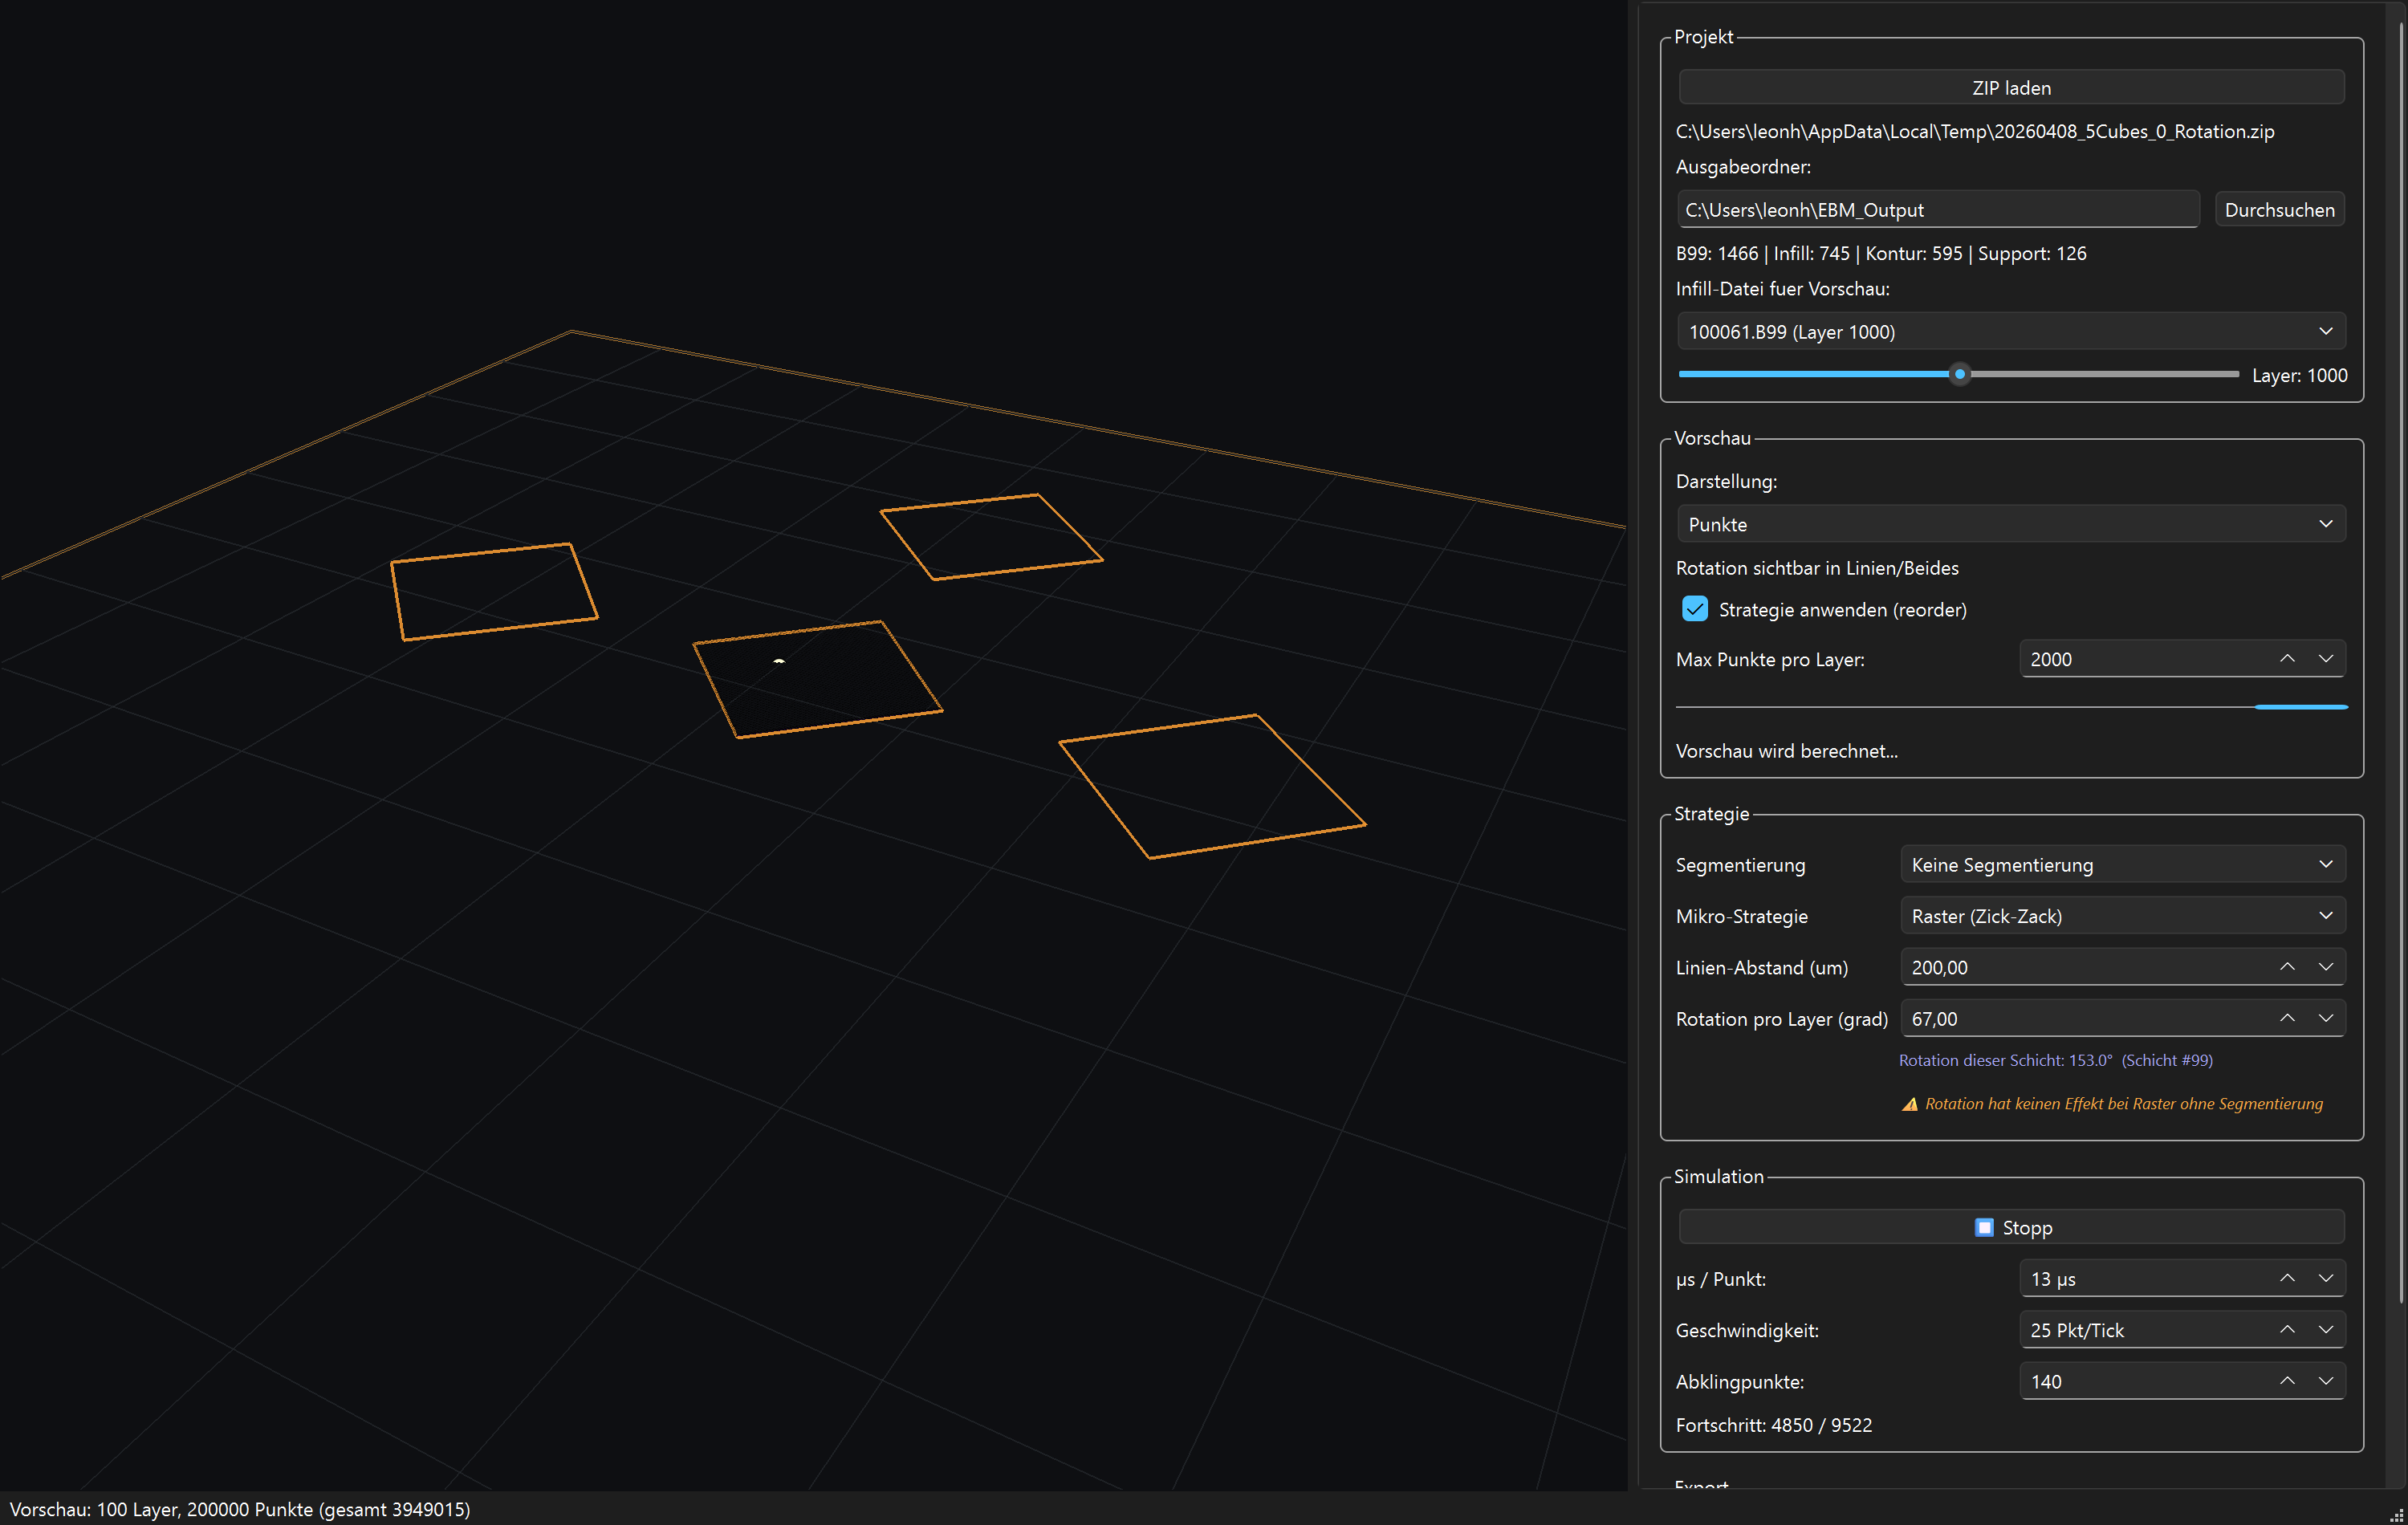
\includegraphics[width=\linewidth]{screenshots/05_simulation.png}
  \caption{Laufende Simulation (herangezoomt). Der helle Punkt markiert die
           aktuelle Strahlposition; die Fortschrittsanzeige zeigt
           \texttt{4850 / 9522}. Über dieselbe Schaltfläche (jetzt
           \texttt{$\blacksquare$ Stopp}) wird die Animation beendet.}
  \label{fig:ebm-sim}
\end{figure}

% ---------------------------------------------------------------------
\subsection{Schritt 4 -- Druckfertiges ZIP exportieren}
\label{subsec:ebm-export}

Ist die Strategie eingestellt, erzeugt die Schaltfläche \textbf{Strategie
anwenden \& ZIP erstellen} im Bereich \emph{Export} das fertige Archiv. Die
Software wendet die gewählte Strategie auf \emph{alle} Infill-Schichten an
(Kontur- und Stützstrukturdateien bleiben unverändert) und legt das Ergebnis
als \texttt{<name>\_NEW.zip} im konfigurierten Ausgabeordner ab. Ein
Fortschrittsbalken zeigt den Verlauf, nach Abschluss erscheint der vollständige
Pfad der erzeugten Datei.

\begin{quote}
  \footnotesize
  Die ursprünglich extrahierten Dateien werden dabei nie verändert. Jeder
  Export arbeitet auf einer frischen Kopie -- ein wiederholter Export liefert
  daher stets dasselbe Ergebnis und es kommt zu keiner doppelten Umsortierung.
\end{quote}

% ---------------------------------------------------------------------
\subsection{Zusammenfassung des Arbeitsablaufs}
\label{subsec:ebm-summary}

\begin{enumerate}
  \item \textbf{ZIP laden} -- Baujob-Archiv mit \texttt{Figure Files/} öffnen.
  \item \textbf{Strategie wählen} -- Segmentierung, Mikro-Strategie und
        Rotation pro Schicht einstellen.
  \item \textbf{Vorschau / Simulation} -- Ergebnis in der 3D-Ansicht prüfen.
  \item \textbf{Export} -- druckfertiges \texttt{*\_NEW.zip} erzeugen.
\end{enumerate}

%
%  Benötigte Pakete (im Hauptdokument in der Präambel):
%     \usepackage{graphicx}
%     \usepackage{booktabs}
%     \usepackage{float}
%     \usepackage{amssymb}               % für ▶/■-Symbole (sonst greift unten ein Fallback)
%     \usepackage[hidelinks]{hyperref}   % optional
%
%  Die Screenshots liegen im Unterordner  screenshots/ .
%  Ggf. den Grafikpfad im Hauptdokument setzen:
%     \graphicspath{{screenshots/}}
%  oder in den \includegraphics-Befehlen den Pfad anpassen.
% =====================================================================

% Fallback: Falls amssymb nicht geladen ist, einfache Ersatzsymbole
% definieren, damit das Dokument trotzdem kompiliert (\triangleright und
% \bullet stammen aus dem LaTeX-Kern und sind immer verfügbar).
\providecommand{\blacktriangleright}{\ensuremath{\triangleright}}
\providecommand{\blacksquare}{\ensuremath{\bullet}}

\section{Bedienung der Software: EBM Strategy Converter}
\label{sec:ebm-anleitung}

Der \emph{EBM Strategy Converter} ist ein Desktop-Werkzeug, das die
Belichtungsreihenfolge (Scan-Strategie) für den Elektronenstrahl-Schmelzprozess
des Arcam~S12 Pro-Beam neu anordnet. Die Software liest ein Baujob-ZIP-Archiv
mit \texttt{.B99}-Punktwolkendateien ein, sortiert die Schmelzpunkte der
Infill-Schichten nach einer frei wählbaren Strategie um und schreibt ein
druckfertiges ZIP zurück. Dabei wird \textbf{keine einzige Koordinate
verändert} -- es ändert sich ausschließlich die \emph{Reihenfolge}, in der die
Punkte belichtet werden.

Die folgende Anleitung beschreibt den Arbeitsablauf in vier Schritten:
ZIP laden $\rightarrow$ Strategie wählen $\rightarrow$ Vorschau prüfen
$\rightarrow$ ZIP exportieren.

% ---------------------------------------------------------------------
\subsection{Überblick über die Oberfläche}
\label{subsec:ebm-overview}

Nach dem Start zeigt das Programm links eine interaktive 3D-Vorschau und rechts
ein Bedien-Panel mit fünf Bereichen: \emph{Projekt}, \emph{Vorschau},
\emph{Strategie}, \emph{Simulation} und \emph{Export}
(Abbildung~\ref{fig:ebm-start}). Die 3D-Ansicht lässt sich mit der Maus drehen
(linke Maustaste) und zoomen (Mausrad).

\begin{figure}[H]
  \centering
  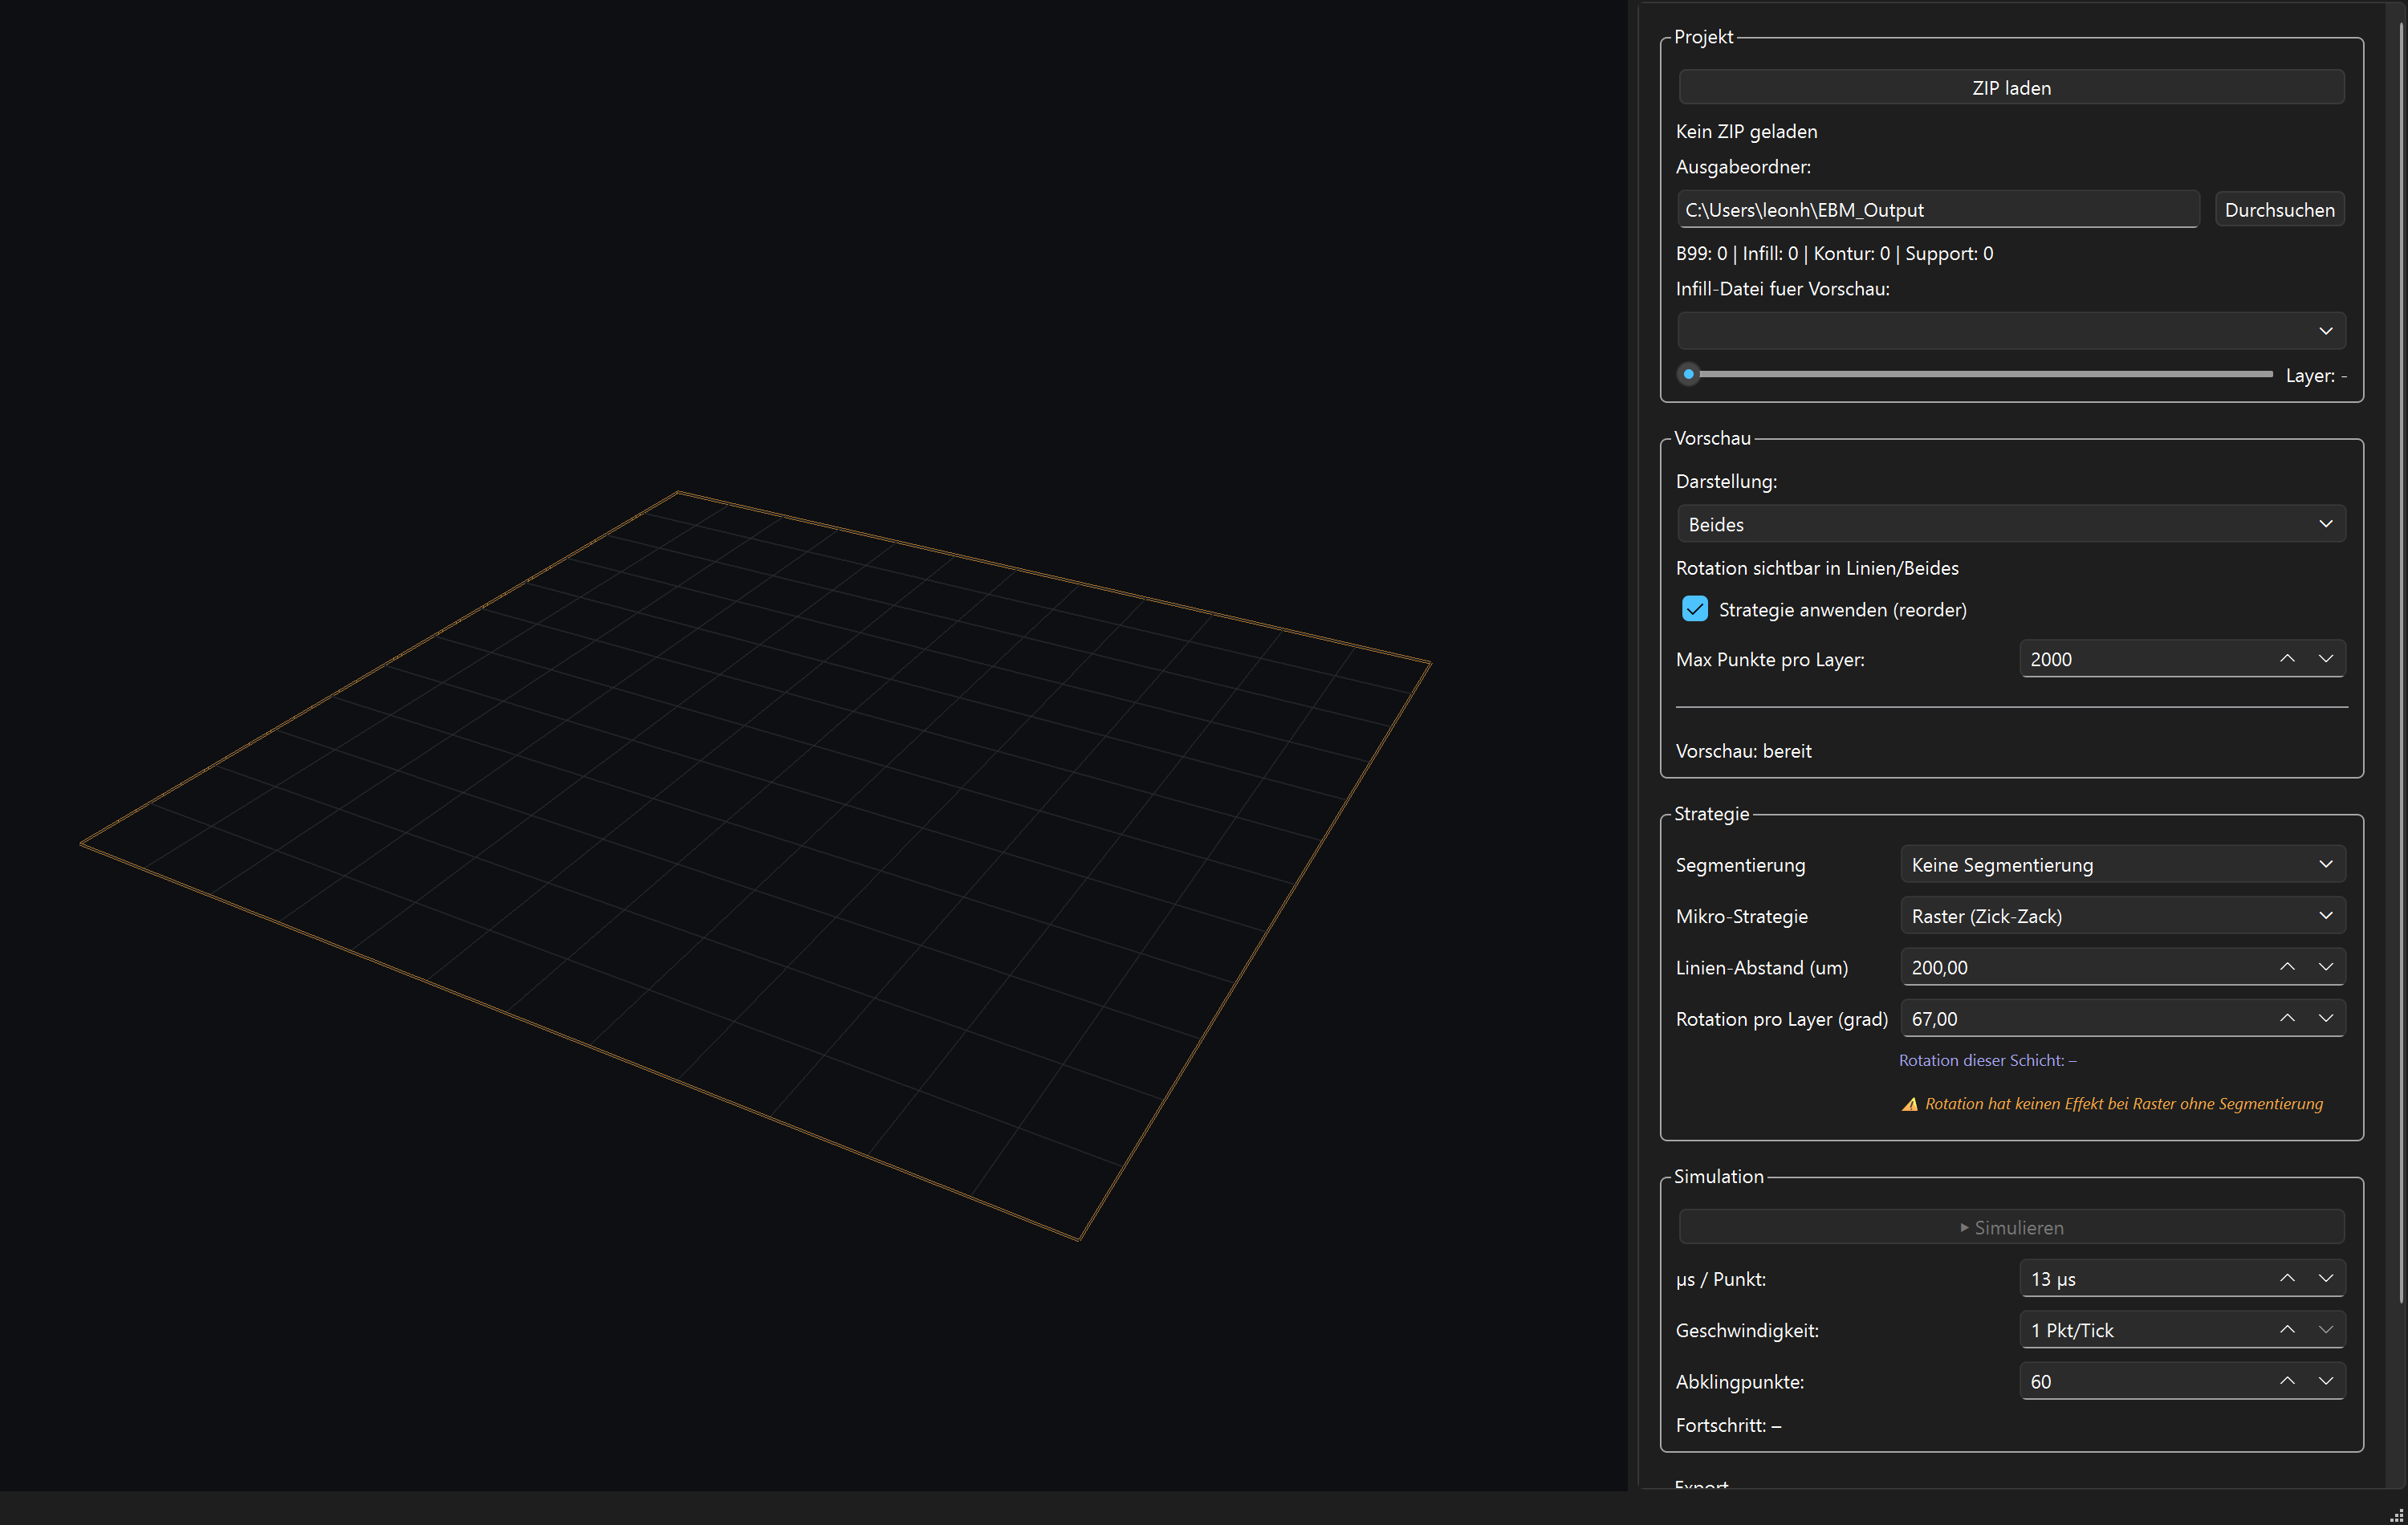
\includegraphics[width=\linewidth]{screenshots/01_startfenster.png}
  \caption{Startfenster nach dem Programmstart. Links die noch leere
           3D-Vorschau (Bauplattform 120\,$\times$\,120\,mm), rechts das
           Bedien-Panel.}
  \label{fig:ebm-start}
\end{figure}

% ---------------------------------------------------------------------
\subsection{Schritt 1 -- Baujob-ZIP laden}
\label{subsec:ebm-load}

Über die Schaltfläche \textbf{ZIP laden} im Bereich \emph{Projekt} wird ein
Baujob-Archiv geöffnet, das einen Ordner \texttt{Figure Files/} mit den
\texttt{.B99}-Dateien enthält (so, wie es die Arcam-Software exportiert). Im
Beispiel wird die Datei \texttt{20260408\_5Cubes\_0\_Rotation.zip}
geladen -- ein Baujob mit fünf Würfeln.

Nach dem Laden klassifiziert die Software alle Dateien automatisch und zeigt
eine Statistik an, z.\,B.\ \texttt{B99: 1466 | Infill: 745 | Kontur: 595 |
Support: 126}. Anschließend erscheint sofort eine 3D-Vorschau der ersten
Infill-Schicht (Abbildung~\ref{fig:ebm-loaded}).

\begin{itemize}
  \item \textbf{Ausgabeordner:} Zielordner für das exportierte ZIP
        (Standard: \texttt{\textasciitilde/EBM\_Output}).
  \item Das Auswahlfeld \textbf{Infill-Datei für Vorschau} und der
        \textbf{Layer-Schieberegler} wählen die anzuzeigende Schicht.
\end{itemize}

\begin{figure}[H]
  \centering
  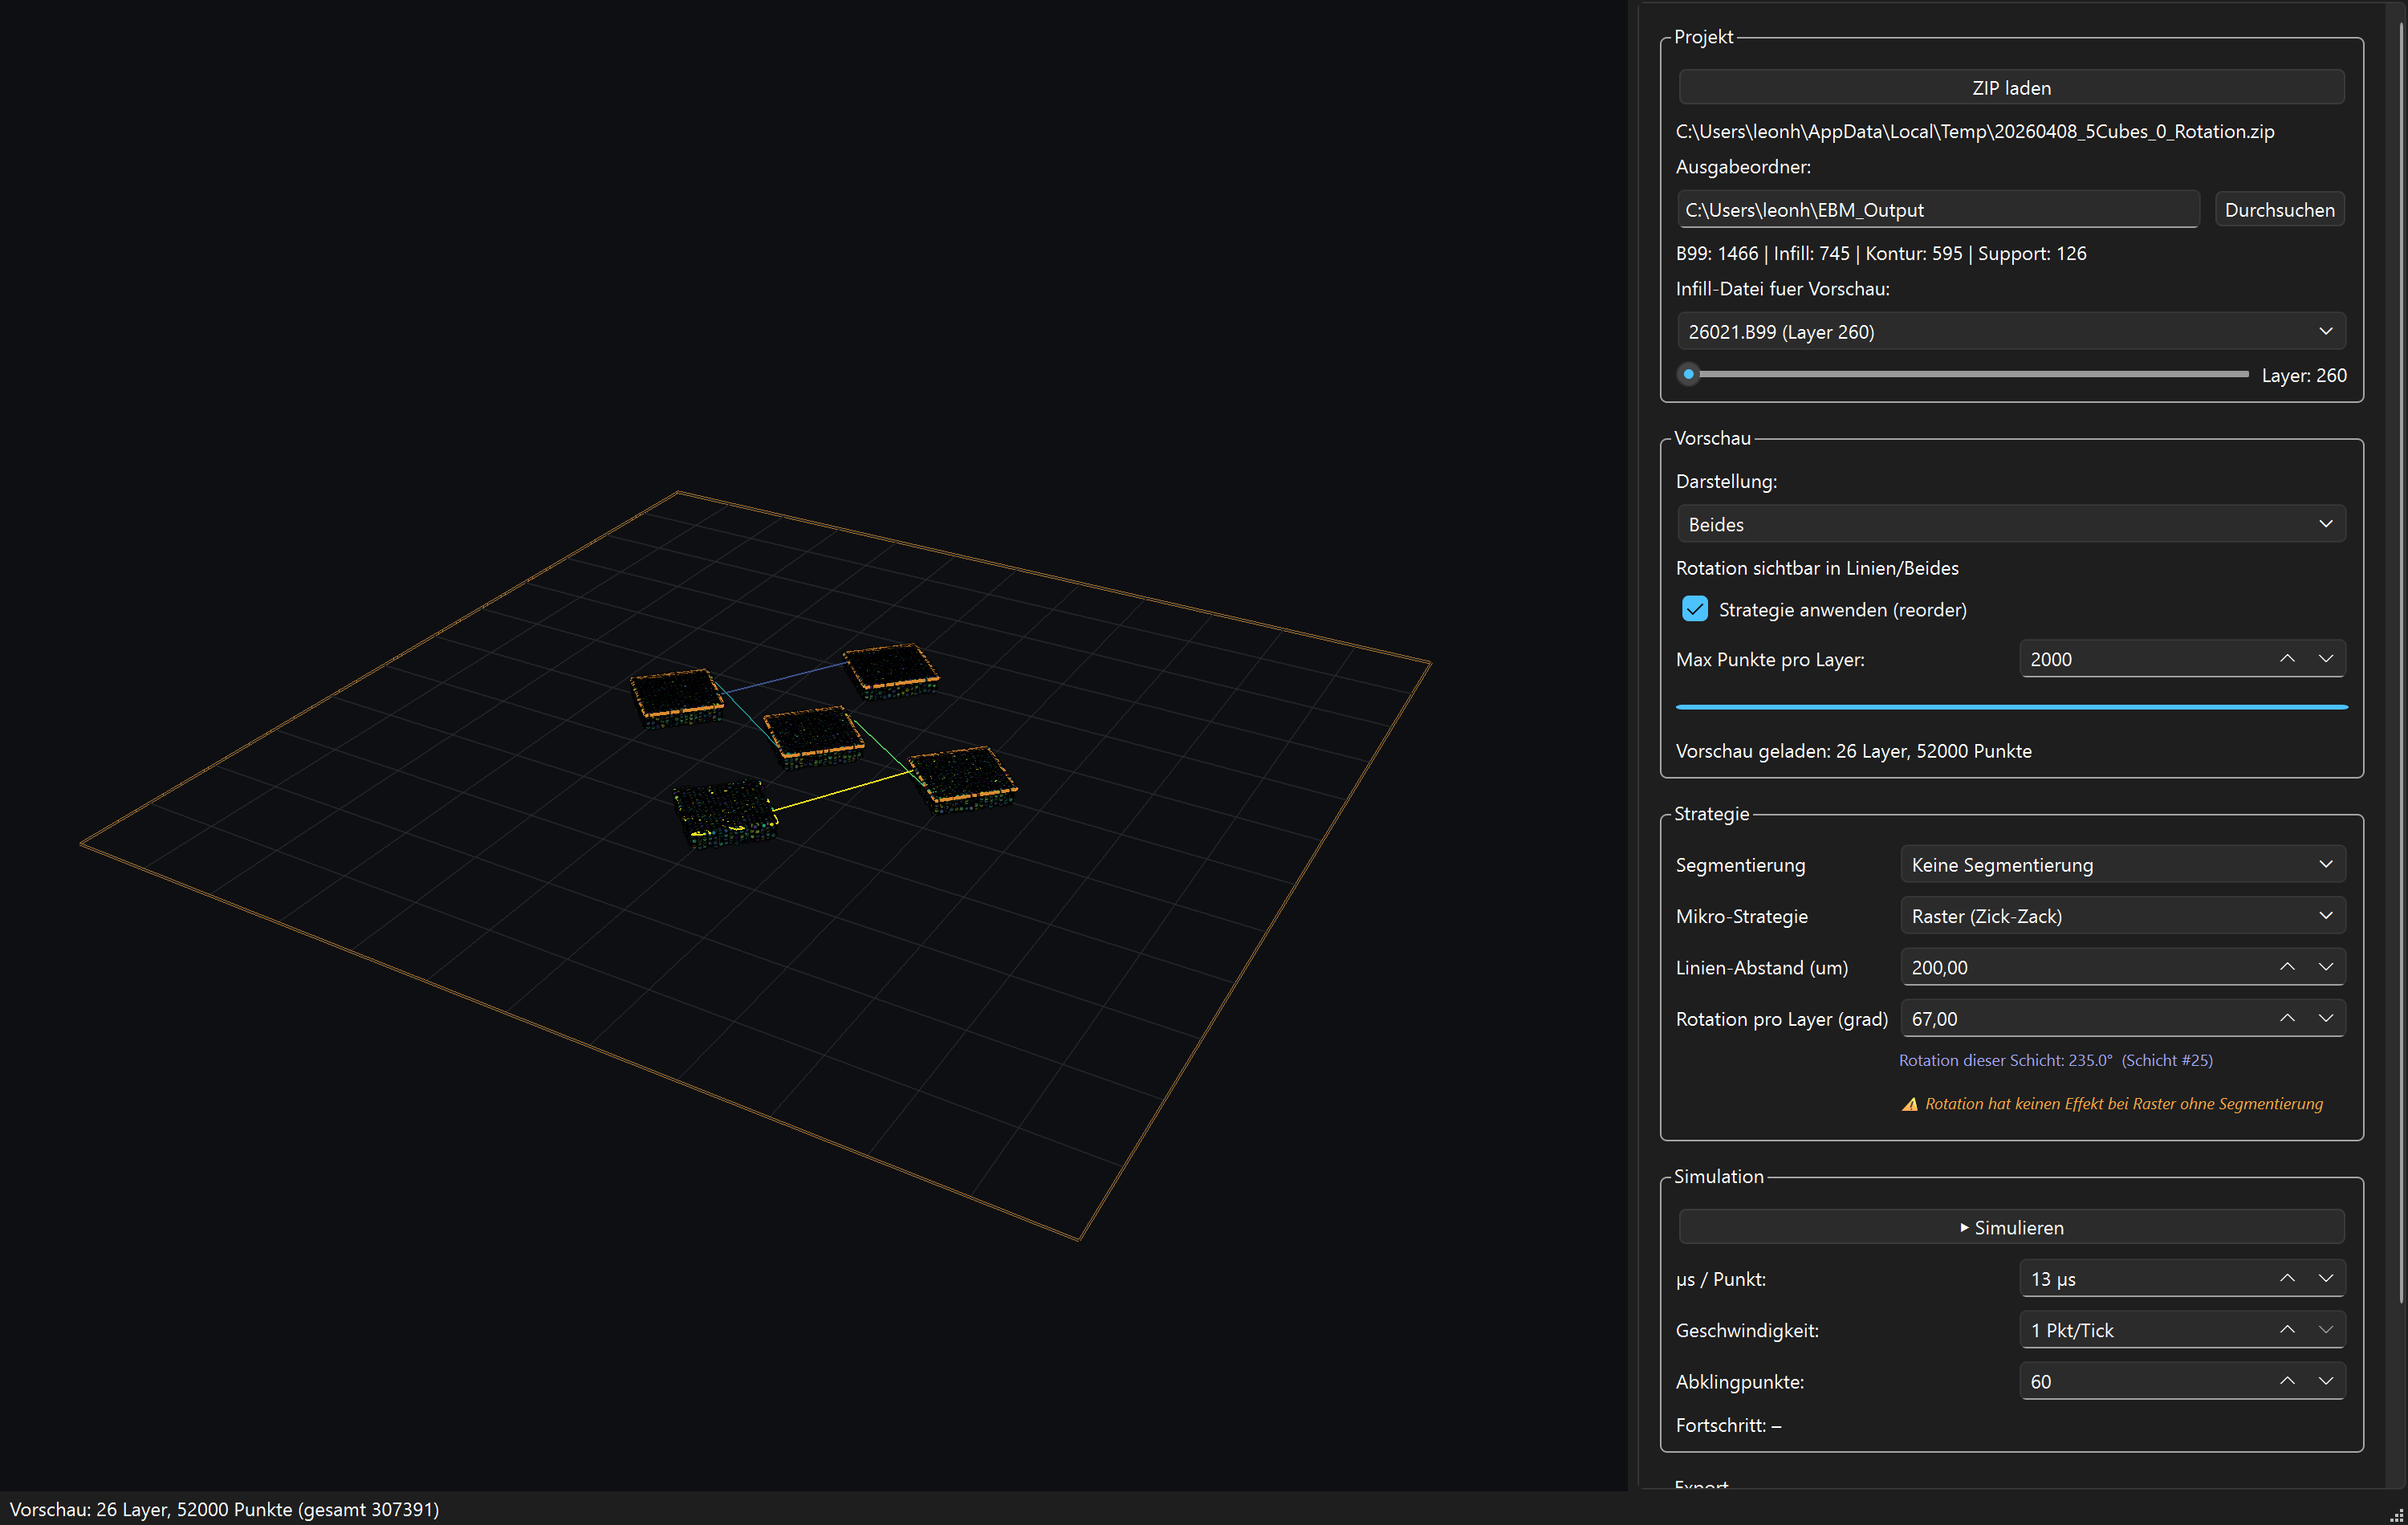
\includegraphics[width=\linewidth]{screenshots/02_projekt_geladen.png}
  \caption{Geladener Baujob. Die fünf Würfel sind als orange Konturen
           erkennbar, die farbigen Punkte zeigen die Infill-Belichtung der
           gewählten Schicht. Oben rechts die Datei-Statistik.}
  \label{fig:ebm-loaded}
\end{figure}

% ---------------------------------------------------------------------
\subsection{Schritt 2 -- Strategie konfigurieren}
\label{subsec:ebm-strategy}

Die Scan-Strategie besteht aus zwei unabhängigen Stufen, die im Bereich
\emph{Strategie} eingestellt werden (Abbildung~\ref{fig:ebm-panel}):

\paragraph{Stufe 1 -- Segmentierung (Makro).}
Legt fest, wie die Schicht grob in Bereiche aufgeteilt wird.

\begin{table}[H]
  \centering
  \begin{tabular}{@{}ll@{}}
    \toprule
    \textbf{Option} & \textbf{Beschreibung} \\
    \midrule
    Keine Segmentierung      & Alle Punkte als ein Block \\
    Schachbrett (Island)     & Quadratische Felder, abwechselnd belichtet \\
    Streifen (Stripe)        & Parallele Bänder \\
    Hexagonal                & Versetztes Waben-Gitter \\
    Spiralzonen              & Konzentrische Ringe um den Schwerpunkt \\
    \bottomrule
  \end{tabular}
  \caption{Verfügbare Segmentierungsarten (Stufe~1).}
  \label{tab:ebm-seg}
\end{table}

\paragraph{Stufe 2 -- Mikro-Strategie.}
Legt fest, in welcher Reihenfolge die Punkte \emph{innerhalb} eines Segments
belichtet werden -- z.\,B.\ \emph{Raster (Zick-Zack)},
\emph{Hilbert-Kurve}, \emph{Spiral} oder \emph{Ghost Beam}. Je nach Auswahl
blendet die Oberfläche die passenden Zusatzparameter ein bzw.\ aus.

\paragraph{Rotation pro Layer.}
Der Wert \emph{Rotation pro Layer (Grad)} dreht das Muster von Schicht zu
Schicht weiter: Schicht~$N$ wird um $N \times \mathrm{Winkel}$ (modulo
$360^\circ$) gedreht. Die Oberfläche zeigt darunter die effektive Rotation der
aktuell gewählten Schicht an (z.\,B.\ \texttt{Rotation dieser Schicht: 153{,}0$^\circ$}).

\begin{quote}
  \footnotesize\itshape
  Hinweis: Bei der Mikro-Strategie \emph{Raster} ohne Segmentierung hat die
  Rotation keinen Effekt -- die Software weist mit einem orangefarbenen
  Warnhinweis darauf hin.
\end{quote}

\begin{figure}[H]
  \centering
  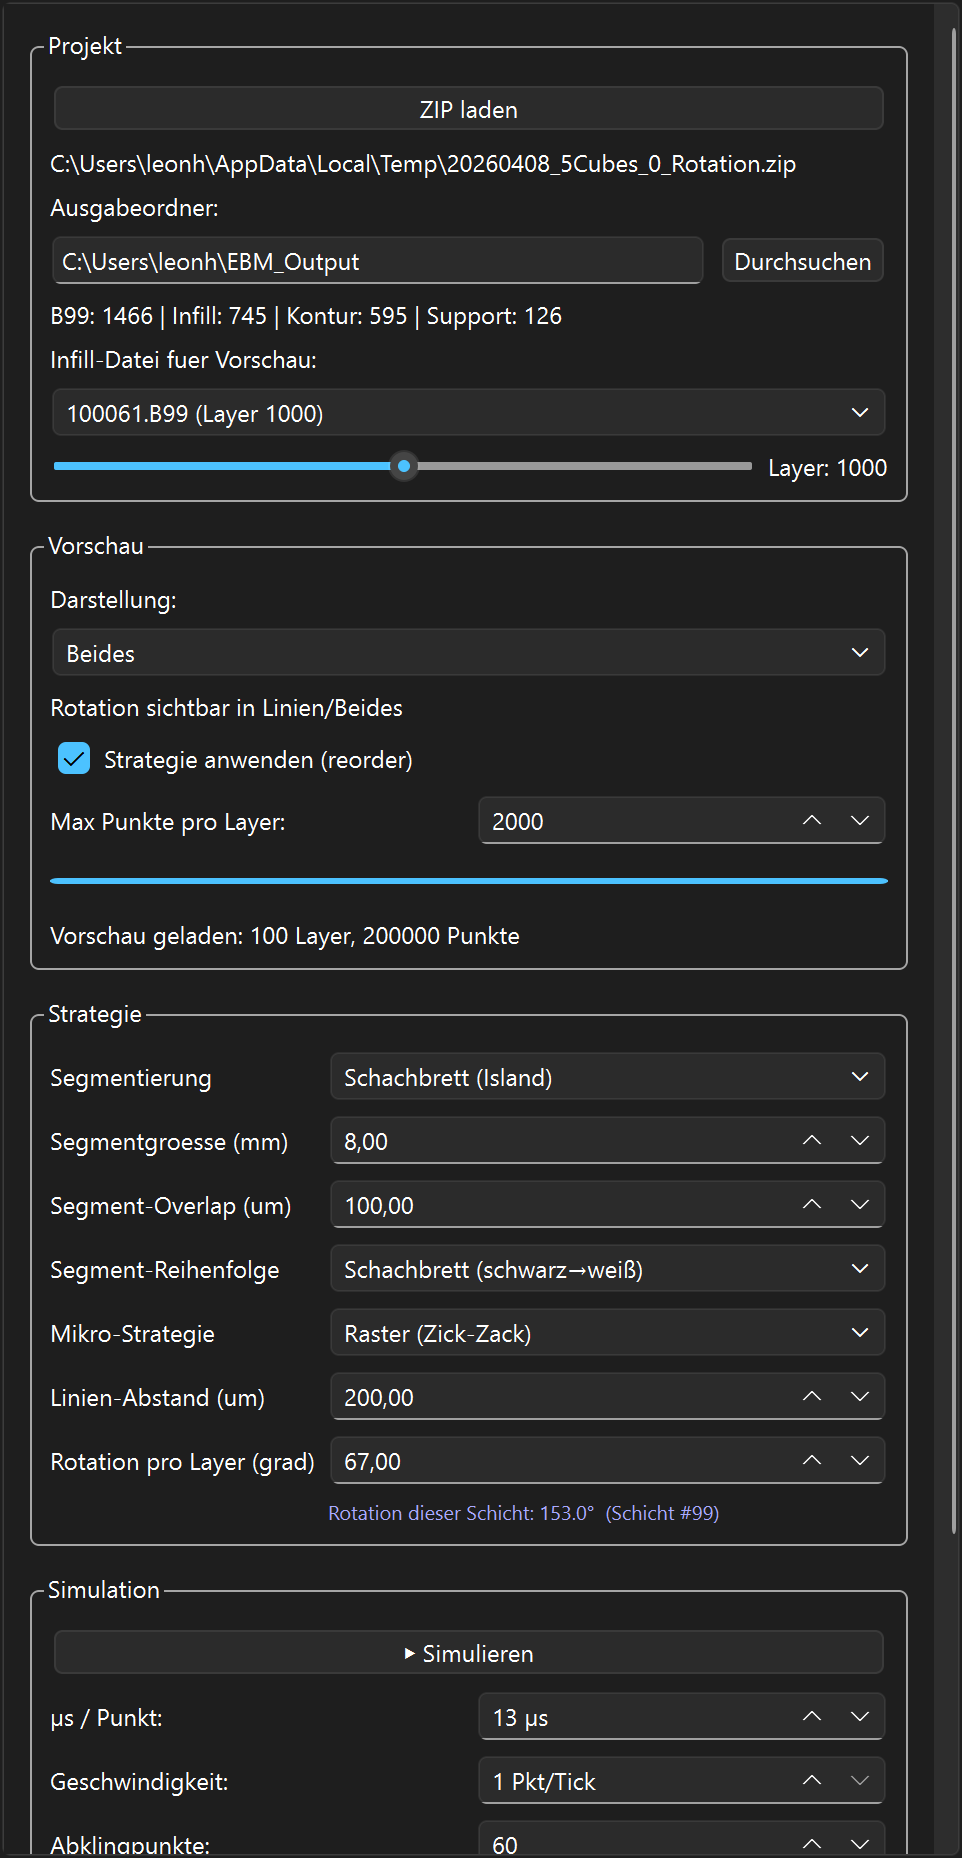
\includegraphics[height=0.82\textheight]{screenshots/04_bedienpanel.png}
  \caption{Das Bedien-Panel im Detail mit konfigurierter
           Schachbrett-Segmentierung und Raster-Mikrostrategie. Unter dem
           Rotationsfeld wird die effektive Rotation der aktuellen Schicht
           angezeigt.}
  \label{fig:ebm-panel}
\end{figure}

% ---------------------------------------------------------------------
\subsection{Schritt 3 -- Vorschau und Simulation prüfen}
\label{subsec:ebm-preview}

Im Bereich \emph{Vorschau} steuert das Feld \textbf{Darstellung} die Ansicht:
\emph{Punkte} zeigt nur die Schmelzpunkte, \emph{Linien} den Scan-Pfad und
\emph{Beides} die Kombination. Mit dem Schieberegler \emph{Layer} lässt sich
durch die Schichten blättern; jede Änderung an der Strategie aktualisiert die
Vorschau automatisch. Abbildung~\ref{fig:ebm-strategy} zeigt die
Schachbrett-Strategie über mehrere übereinanderliegende Schichten, wodurch die
schichtweise Rotation sichtbar wird.

\begin{figure}[H]
  \centering
  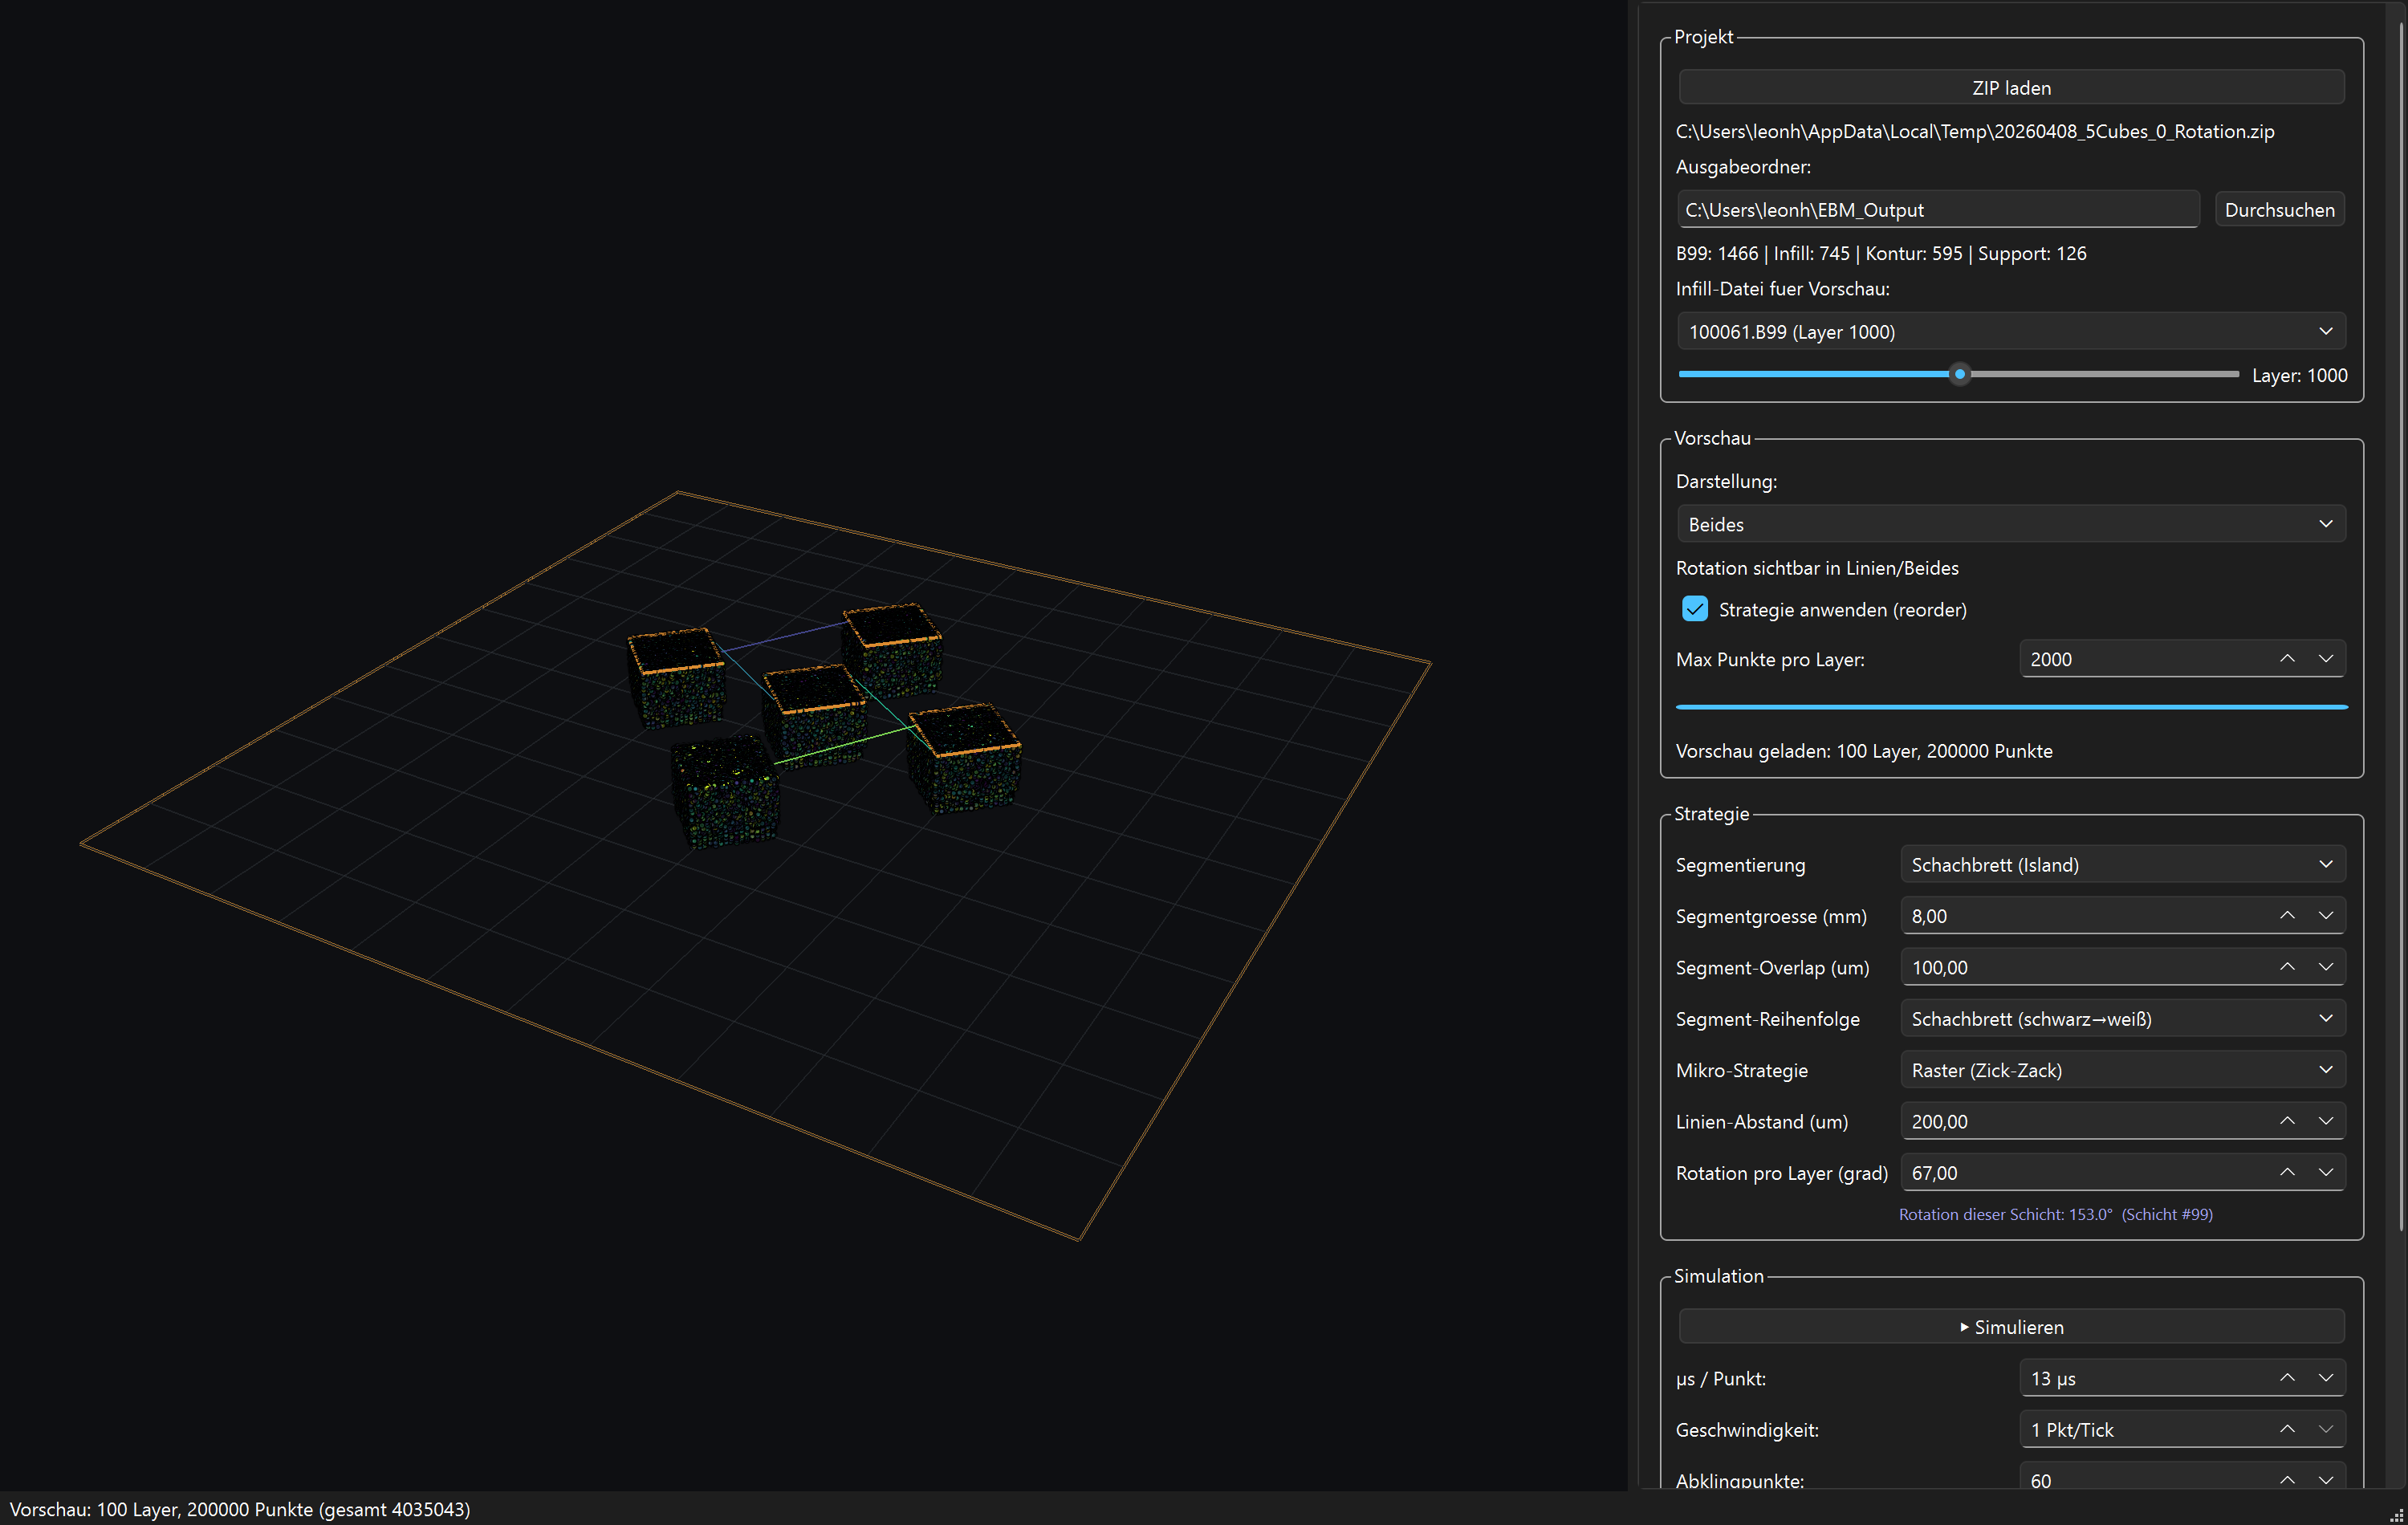
\includegraphics[width=\linewidth]{screenshots/03_strategie_vorschau.png}
  \caption{3D-Vorschau mit aktiver Schachbrett-Segmentierung und
           schichtweiser Rotation. Die grünen Linien zeigen den Scan-Pfad der
           aktuell gewählten Schicht.}
  \label{fig:ebm-strategy}
\end{figure}

\paragraph{Simulation.}
Über \textbf{$\blacktriangleright$~Simulieren} im Bereich \emph{Simulation}
wird die Belichtung der gewählten Schicht Punkt für Punkt animiert. Der gerade
belichtete Punkt leuchtet hell auf, bereits belichtete Punkte klingen langsam
ab -- so wird die Reihenfolge der Strategie unmittelbar nachvollziehbar
(Abbildung~\ref{fig:ebm-sim}). Die Parameter steuern das Tempo:

\begin{itemize}
  \item \textbf{$\mu$s / Punkt} -- realistische Haltezeit pro Punkt
        (typisch 13\,$\mu$s).
  \item \textbf{Geschwindigkeit (Pkt/Tick)} -- wie viele Punkte pro Animations-
        schritt gezeichnet werden; höhere Werte beschleunigen den Durchlauf.
  \item \textbf{Abklingpunkte} -- Länge der nachleuchtenden Spur.
\end{itemize}

\begin{figure}[H]
  \centering
  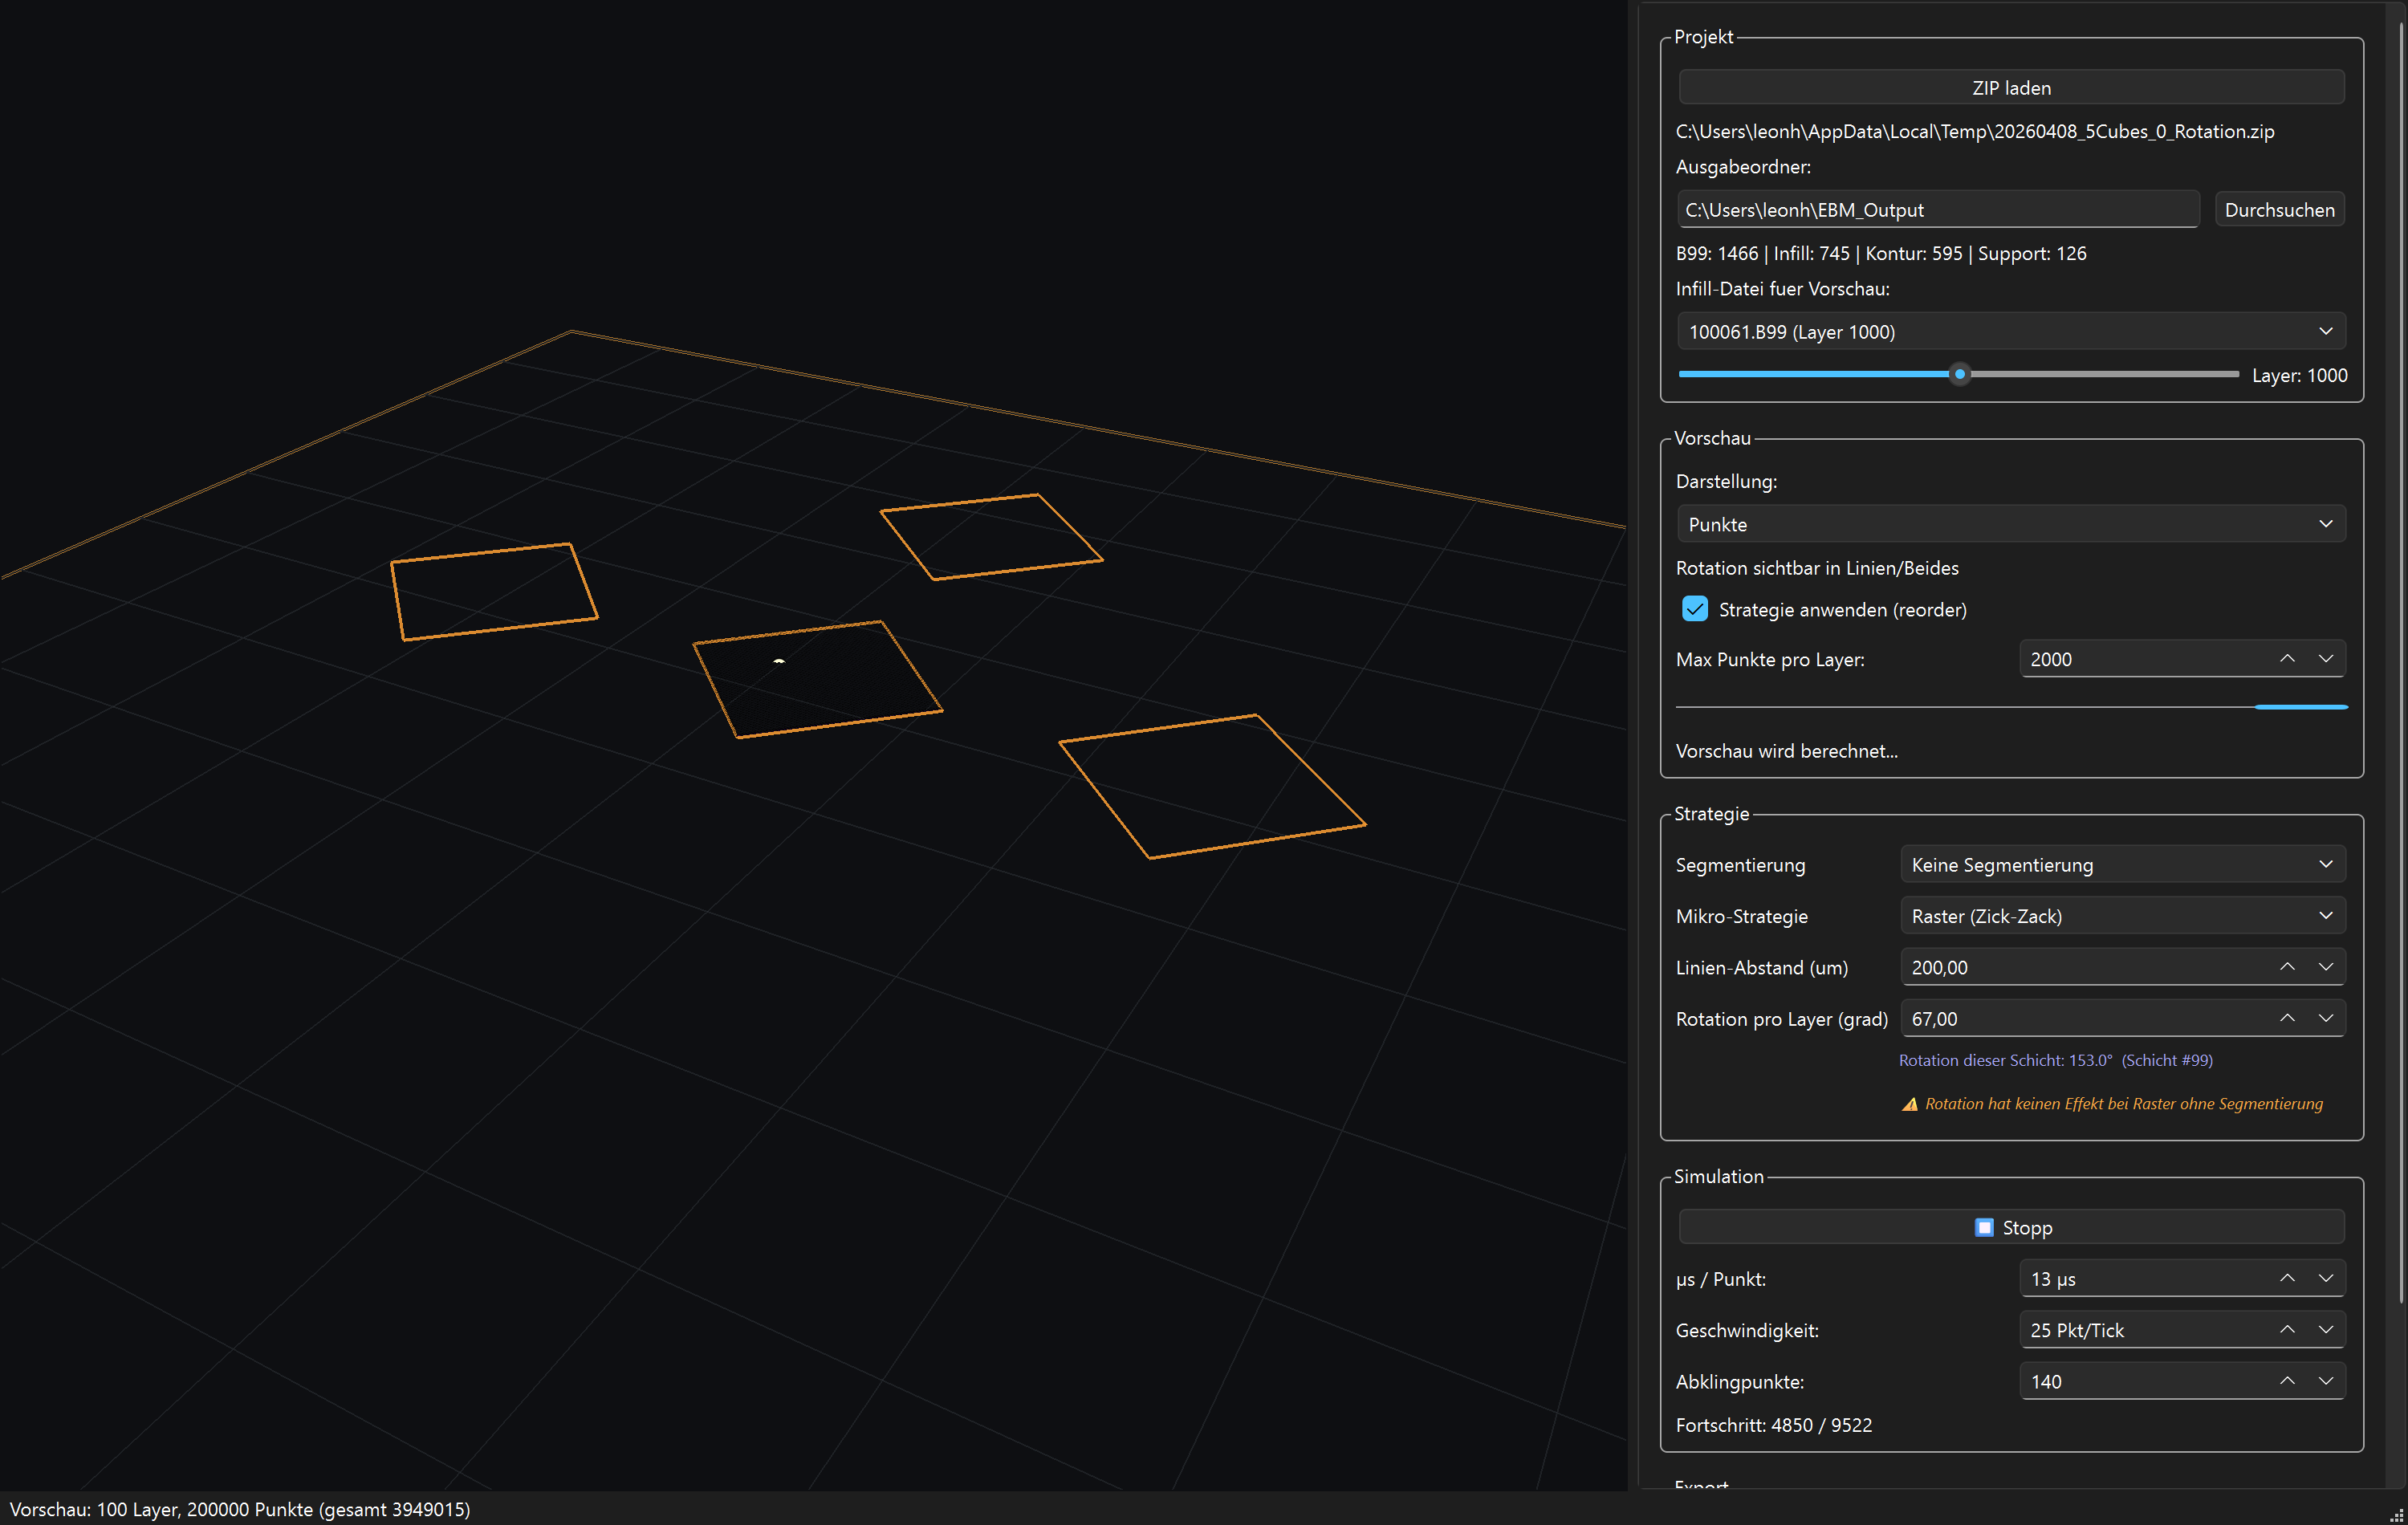
\includegraphics[width=\linewidth]{screenshots/05_simulation.png}
  \caption{Laufende Simulation (herangezoomt). Der helle Punkt markiert die
           aktuelle Strahlposition; die Fortschrittsanzeige zeigt
           \texttt{4850 / 9522}. Über dieselbe Schaltfläche (jetzt
           \texttt{$\blacksquare$ Stopp}) wird die Animation beendet.}
  \label{fig:ebm-sim}
\end{figure}

% ---------------------------------------------------------------------
\subsection{Schritt 4 -- Druckfertiges ZIP exportieren}
\label{subsec:ebm-export}

Ist die Strategie eingestellt, erzeugt die Schaltfläche \textbf{Strategie
anwenden \& ZIP erstellen} im Bereich \emph{Export} das fertige Archiv. Die
Software wendet die gewählte Strategie auf \emph{alle} Infill-Schichten an
(Kontur- und Stützstrukturdateien bleiben unverändert) und legt das Ergebnis
als \texttt{<name>\_NEW.zip} im konfigurierten Ausgabeordner ab. Ein
Fortschrittsbalken zeigt den Verlauf, nach Abschluss erscheint der vollständige
Pfad der erzeugten Datei.

\begin{quote}
  \footnotesize
  Die ursprünglich extrahierten Dateien werden dabei nie verändert. Jeder
  Export arbeitet auf einer frischen Kopie -- ein wiederholter Export liefert
  daher stets dasselbe Ergebnis und es kommt zu keiner doppelten Umsortierung.
\end{quote}

% ---------------------------------------------------------------------
\subsection{Zusammenfassung des Arbeitsablaufs}
\label{subsec:ebm-summary}

\begin{enumerate}
  \item \textbf{ZIP laden} -- Baujob-Archiv mit \texttt{Figure Files/} öffnen.
  \item \textbf{Strategie wählen} -- Segmentierung, Mikro-Strategie und
        Rotation pro Schicht einstellen.
  \item \textbf{Vorschau / Simulation} -- Ergebnis in der 3D-Ansicht prüfen.
  \item \textbf{Export} -- druckfertiges \texttt{*\_NEW.zip} erzeugen.
\end{enumerate}

%
%  Benötigte Pakete (im Hauptdokument in der Präambel):
%     \usepackage{graphicx}
%     \usepackage{booktabs}
%     \usepackage{float}
%     \usepackage{amssymb}               % für ▶/■-Symbole (sonst greift unten ein Fallback)
%     \usepackage[hidelinks]{hyperref}   % optional
%
%  Die Screenshots liegen im Unterordner  screenshots/ .
%  Ggf. den Grafikpfad im Hauptdokument setzen:
%     \graphicspath{{screenshots/}}
%  oder in den \includegraphics-Befehlen den Pfad anpassen.
% =====================================================================

% Fallback: Falls amssymb nicht geladen ist, einfache Ersatzsymbole
% definieren, damit das Dokument trotzdem kompiliert (\triangleright und
% \bullet stammen aus dem LaTeX-Kern und sind immer verfügbar).
\providecommand{\blacktriangleright}{\ensuremath{\triangleright}}
\providecommand{\blacksquare}{\ensuremath{\bullet}}

\section{Bedienung der Software: EBM Strategy Converter}
\label{sec:ebm-anleitung}

Der \emph{EBM Strategy Converter} ist ein Desktop-Werkzeug, das die
Belichtungsreihenfolge (Scan-Strategie) für den Elektronenstrahl-Schmelzprozess
des Arcam~S12 Pro-Beam neu anordnet. Die Software liest ein Baujob-ZIP-Archiv
mit \texttt{.B99}-Punktwolkendateien ein, sortiert die Schmelzpunkte der
Infill-Schichten nach einer frei wählbaren Strategie um und schreibt ein
druckfertiges ZIP zurück. Dabei wird \textbf{keine einzige Koordinate
verändert} -- es ändert sich ausschließlich die \emph{Reihenfolge}, in der die
Punkte belichtet werden.

Die folgende Anleitung beschreibt den Arbeitsablauf in vier Schritten:
ZIP laden $\rightarrow$ Strategie wählen $\rightarrow$ Vorschau prüfen
$\rightarrow$ ZIP exportieren.

% ---------------------------------------------------------------------
\subsection{Überblick über die Oberfläche}
\label{subsec:ebm-overview}

Nach dem Start zeigt das Programm links eine interaktive 3D-Vorschau und rechts
ein Bedien-Panel mit fünf Bereichen: \emph{Projekt}, \emph{Vorschau},
\emph{Strategie}, \emph{Simulation} und \emph{Export}
(Abbildung~\ref{fig:ebm-start}). Die 3D-Ansicht lässt sich mit der Maus drehen
(linke Maustaste) und zoomen (Mausrad).

\begin{figure}[H]
  \centering
  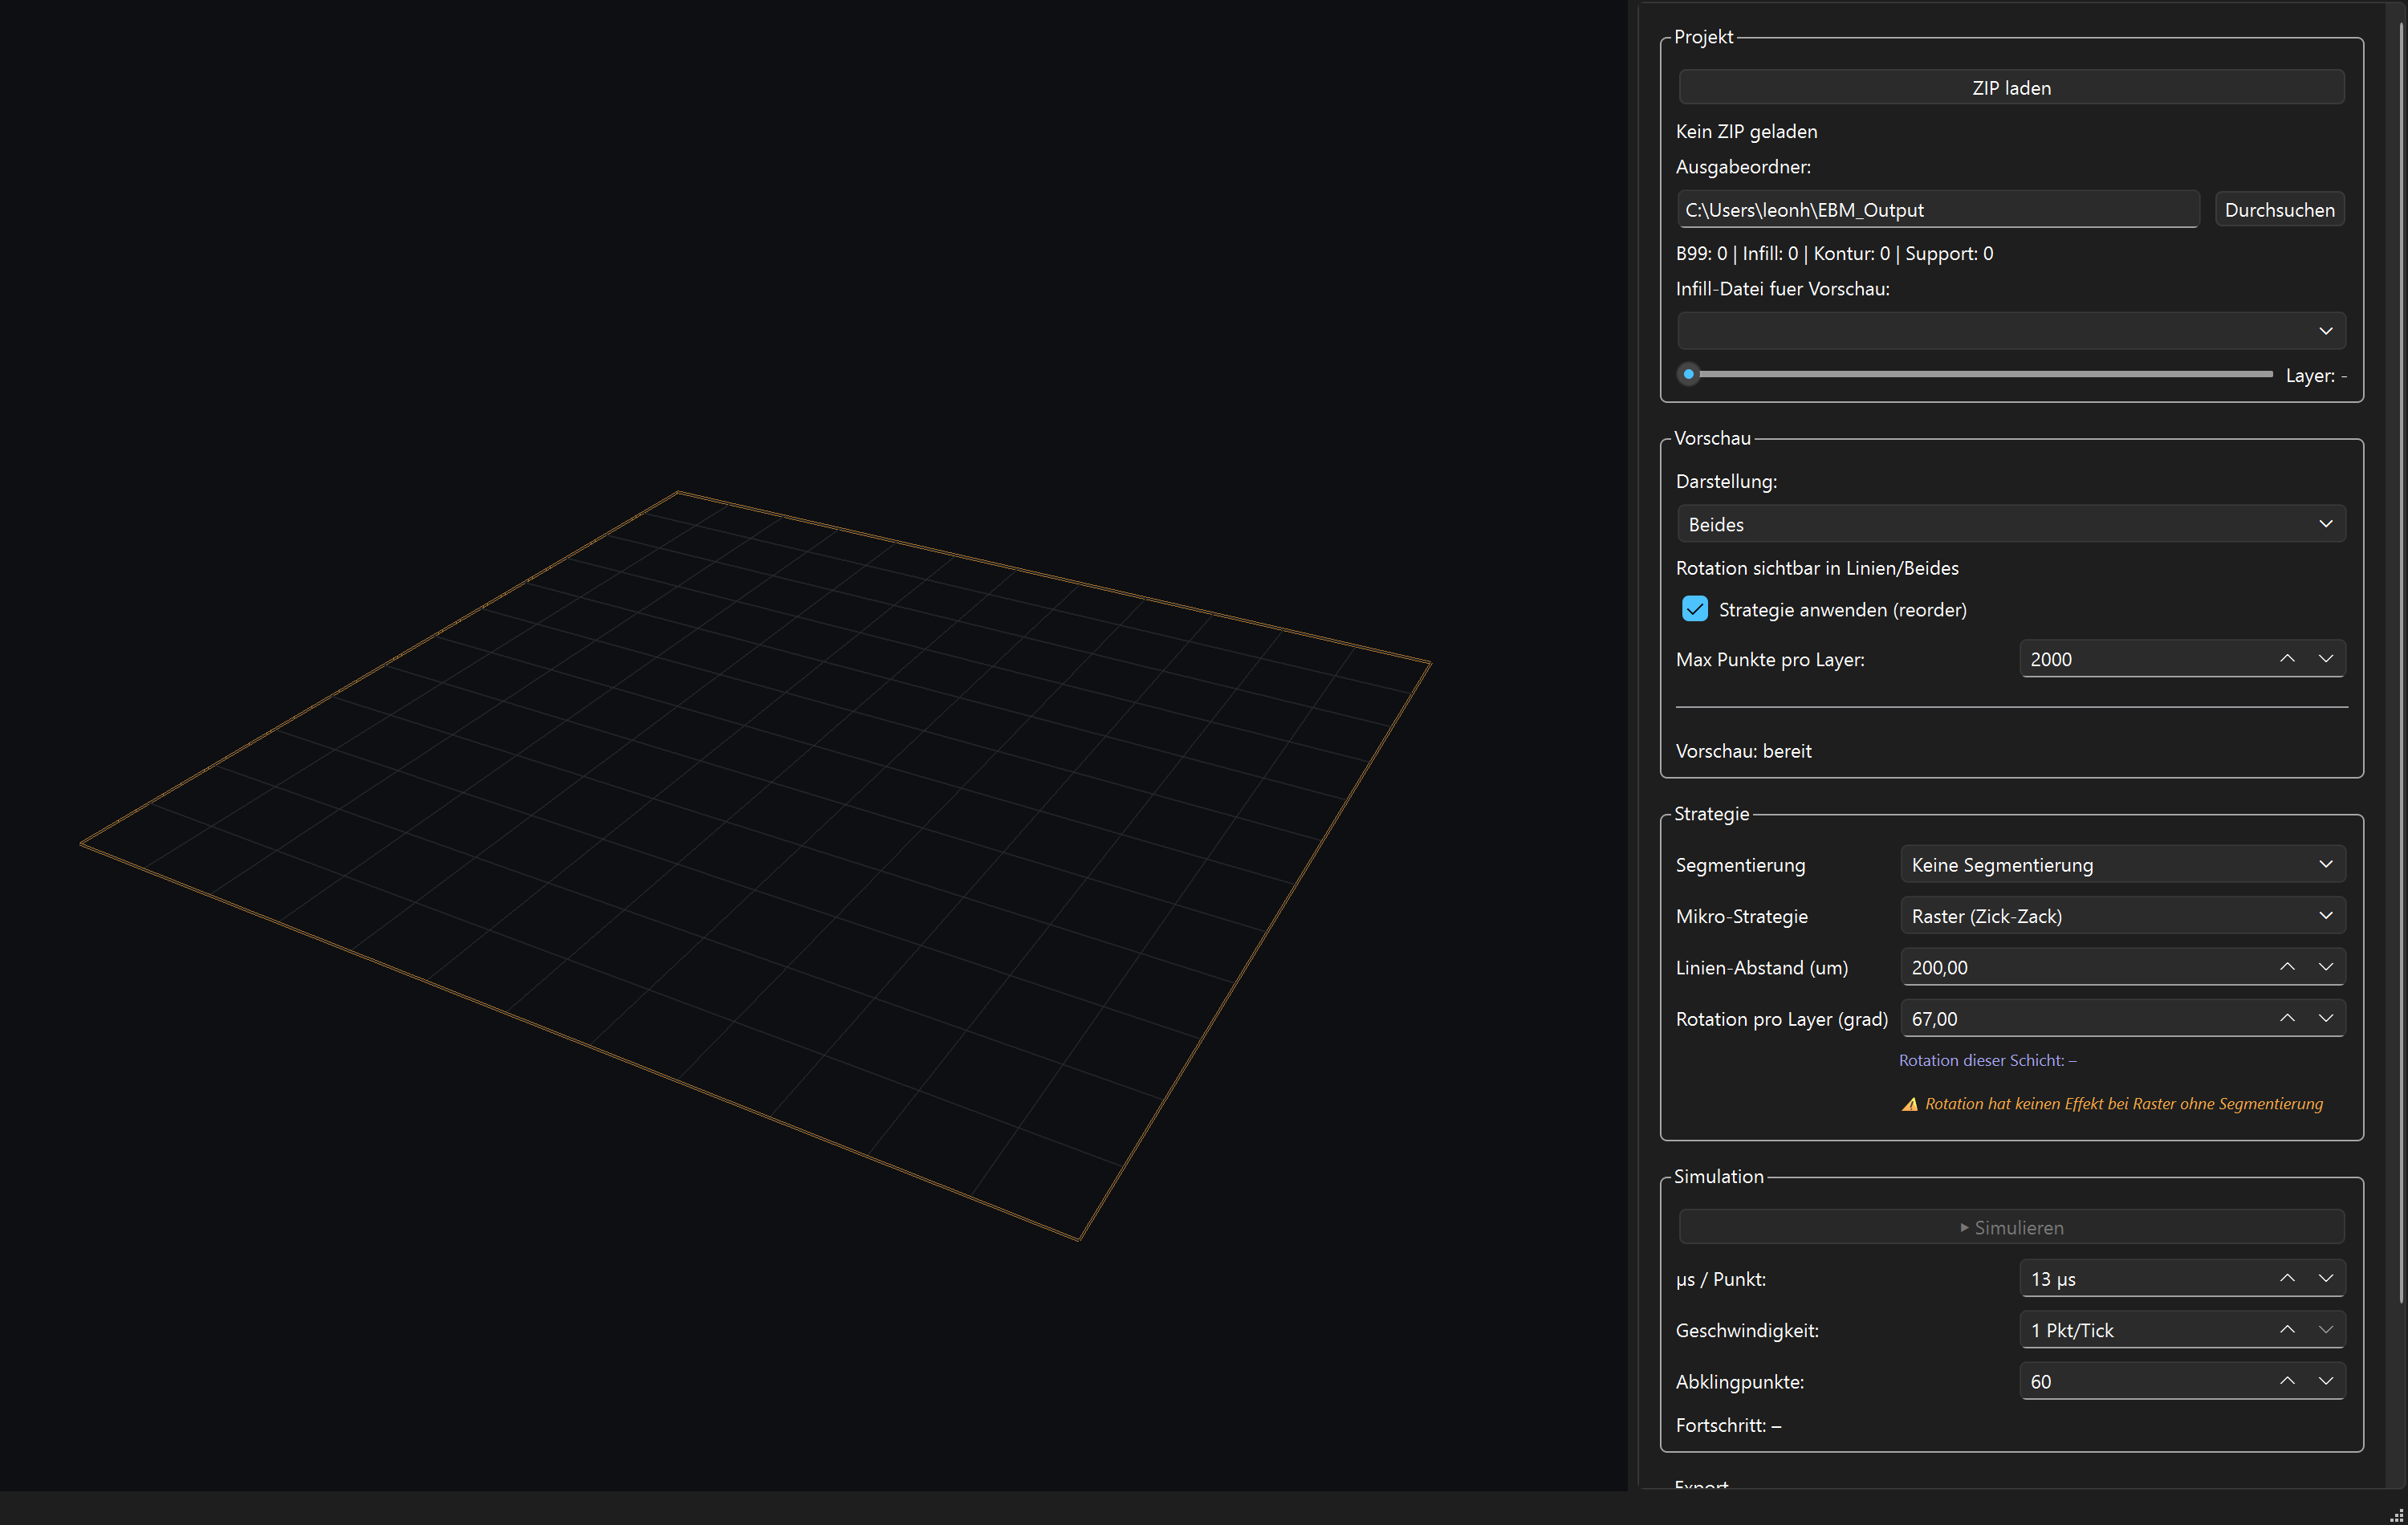
\includegraphics[width=\linewidth]{screenshots/01_startfenster.png}
  \caption{Startfenster nach dem Programmstart. Links die noch leere
           3D-Vorschau (Bauplattform 120\,$\times$\,120\,mm), rechts das
           Bedien-Panel.}
  \label{fig:ebm-start}
\end{figure}

% ---------------------------------------------------------------------
\subsection{Schritt 1 -- Baujob-ZIP laden}
\label{subsec:ebm-load}

Über die Schaltfläche \textbf{ZIP laden} im Bereich \emph{Projekt} wird ein
Baujob-Archiv geöffnet, das einen Ordner \texttt{Figure Files/} mit den
\texttt{.B99}-Dateien enthält (so, wie es die Arcam-Software exportiert). Im
Beispiel wird die Datei \texttt{20260408\_5Cubes\_0\_Rotation.zip}
geladen -- ein Baujob mit fünf Würfeln.

Nach dem Laden klassifiziert die Software alle Dateien automatisch und zeigt
eine Statistik an, z.\,B.\ \texttt{B99: 1466 | Infill: 745 | Kontur: 595 |
Support: 126}. Anschließend erscheint sofort eine 3D-Vorschau der ersten
Infill-Schicht (Abbildung~\ref{fig:ebm-loaded}).

\begin{itemize}
  \item \textbf{Ausgabeordner:} Zielordner für das exportierte ZIP
        (Standard: \texttt{\textasciitilde/EBM\_Output}).
  \item Das Auswahlfeld \textbf{Infill-Datei für Vorschau} und der
        \textbf{Layer-Schieberegler} wählen die anzuzeigende Schicht.
\end{itemize}

\begin{figure}[H]
  \centering
  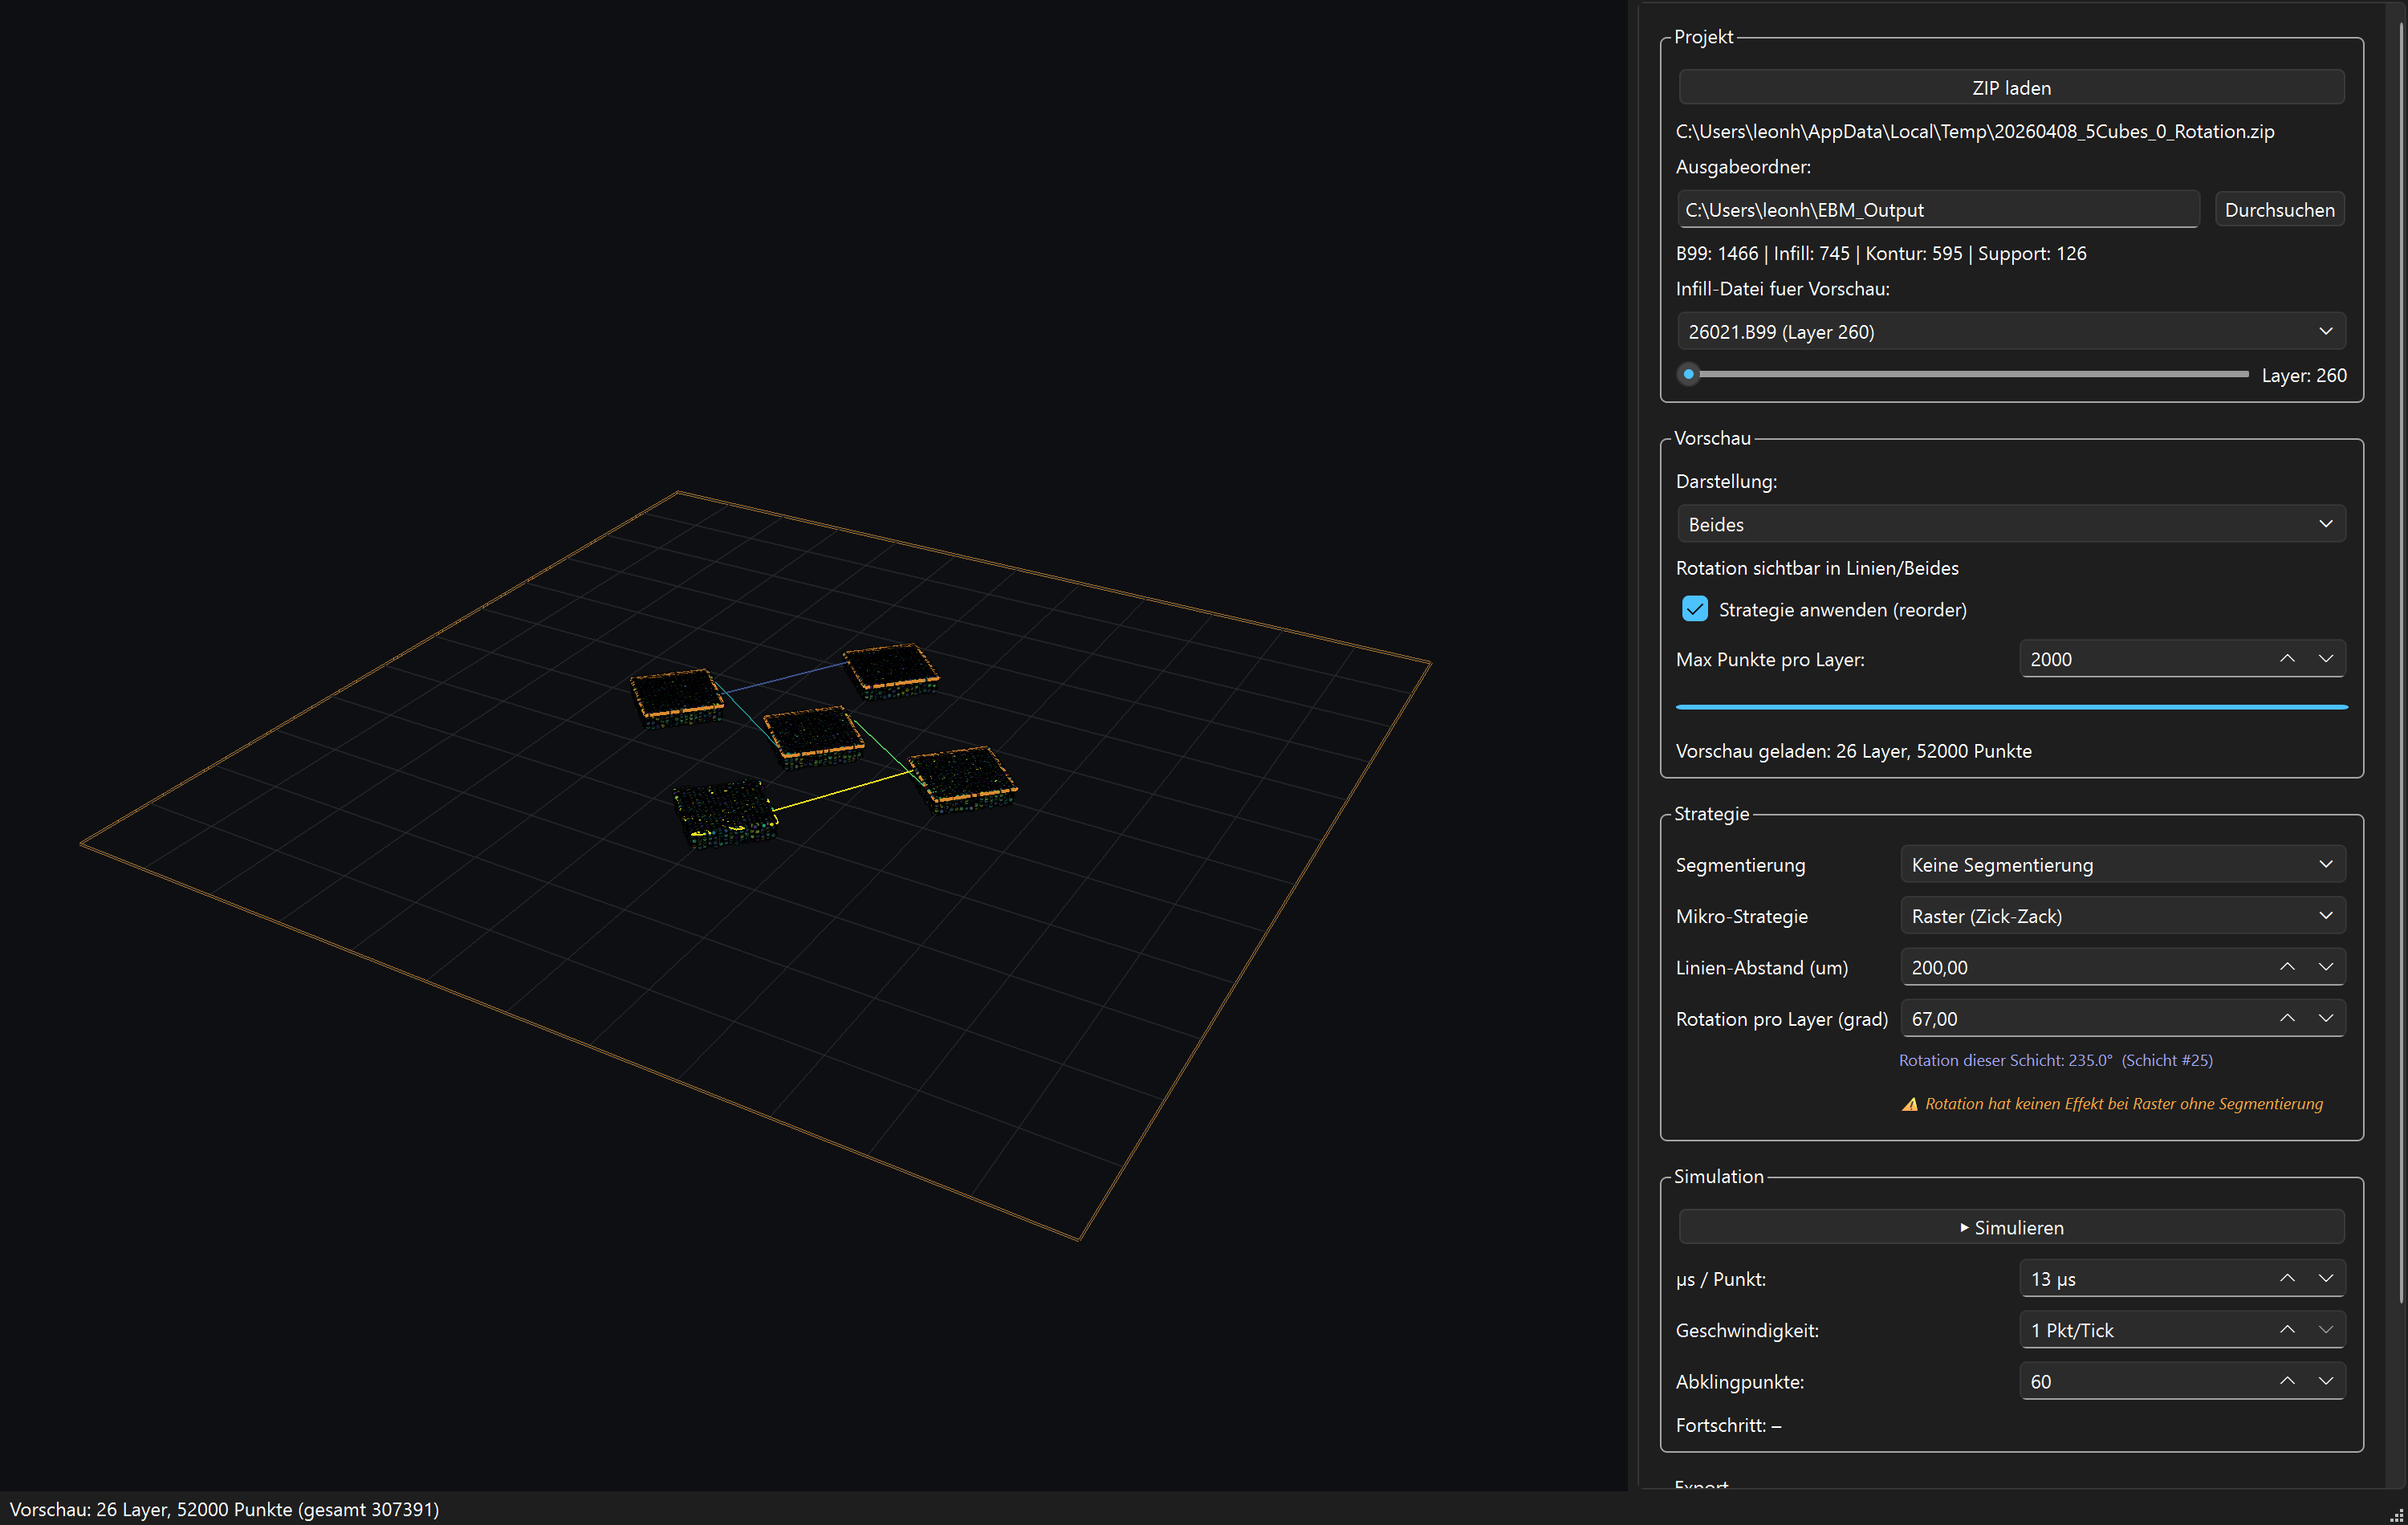
\includegraphics[width=\linewidth]{screenshots/02_projekt_geladen.png}
  \caption{Geladener Baujob. Die fünf Würfel sind als orange Konturen
           erkennbar, die farbigen Punkte zeigen die Infill-Belichtung der
           gewählten Schicht. Oben rechts die Datei-Statistik.}
  \label{fig:ebm-loaded}
\end{figure}

% ---------------------------------------------------------------------
\subsection{Schritt 2 -- Strategie konfigurieren}
\label{subsec:ebm-strategy}

Die Scan-Strategie besteht aus zwei unabhängigen Stufen, die im Bereich
\emph{Strategie} eingestellt werden (Abbildung~\ref{fig:ebm-panel}):

\paragraph{Stufe 1 -- Segmentierung (Makro).}
Legt fest, wie die Schicht grob in Bereiche aufgeteilt wird.

\begin{table}[H]
  \centering
  \begin{tabular}{@{}ll@{}}
    \toprule
    \textbf{Option} & \textbf{Beschreibung} \\
    \midrule
    Keine Segmentierung      & Alle Punkte als ein Block \\
    Schachbrett (Island)     & Quadratische Felder, abwechselnd belichtet \\
    Streifen (Stripe)        & Parallele Bänder \\
    Hexagonal                & Versetztes Waben-Gitter \\
    Spiralzonen              & Konzentrische Ringe um den Schwerpunkt \\
    \bottomrule
  \end{tabular}
  \caption{Verfügbare Segmentierungsarten (Stufe~1).}
  \label{tab:ebm-seg}
\end{table}

\paragraph{Stufe 2 -- Mikro-Strategie.}
Legt fest, in welcher Reihenfolge die Punkte \emph{innerhalb} eines Segments
belichtet werden -- z.\,B.\ \emph{Raster (Zick-Zack)},
\emph{Hilbert-Kurve}, \emph{Spiral} oder \emph{Ghost Beam}. Je nach Auswahl
blendet die Oberfläche die passenden Zusatzparameter ein bzw.\ aus.

\paragraph{Rotation pro Layer.}
Der Wert \emph{Rotation pro Layer (Grad)} dreht das Muster von Schicht zu
Schicht weiter: Schicht~$N$ wird um $N \times \mathrm{Winkel}$ (modulo
$360^\circ$) gedreht. Die Oberfläche zeigt darunter die effektive Rotation der
aktuell gewählten Schicht an (z.\,B.\ \texttt{Rotation dieser Schicht: 153{,}0$^\circ$}).

\begin{quote}
  \footnotesize\itshape
  Hinweis: Bei der Mikro-Strategie \emph{Raster} ohne Segmentierung hat die
  Rotation keinen Effekt -- die Software weist mit einem orangefarbenen
  Warnhinweis darauf hin.
\end{quote}

\begin{figure}[H]
  \centering
  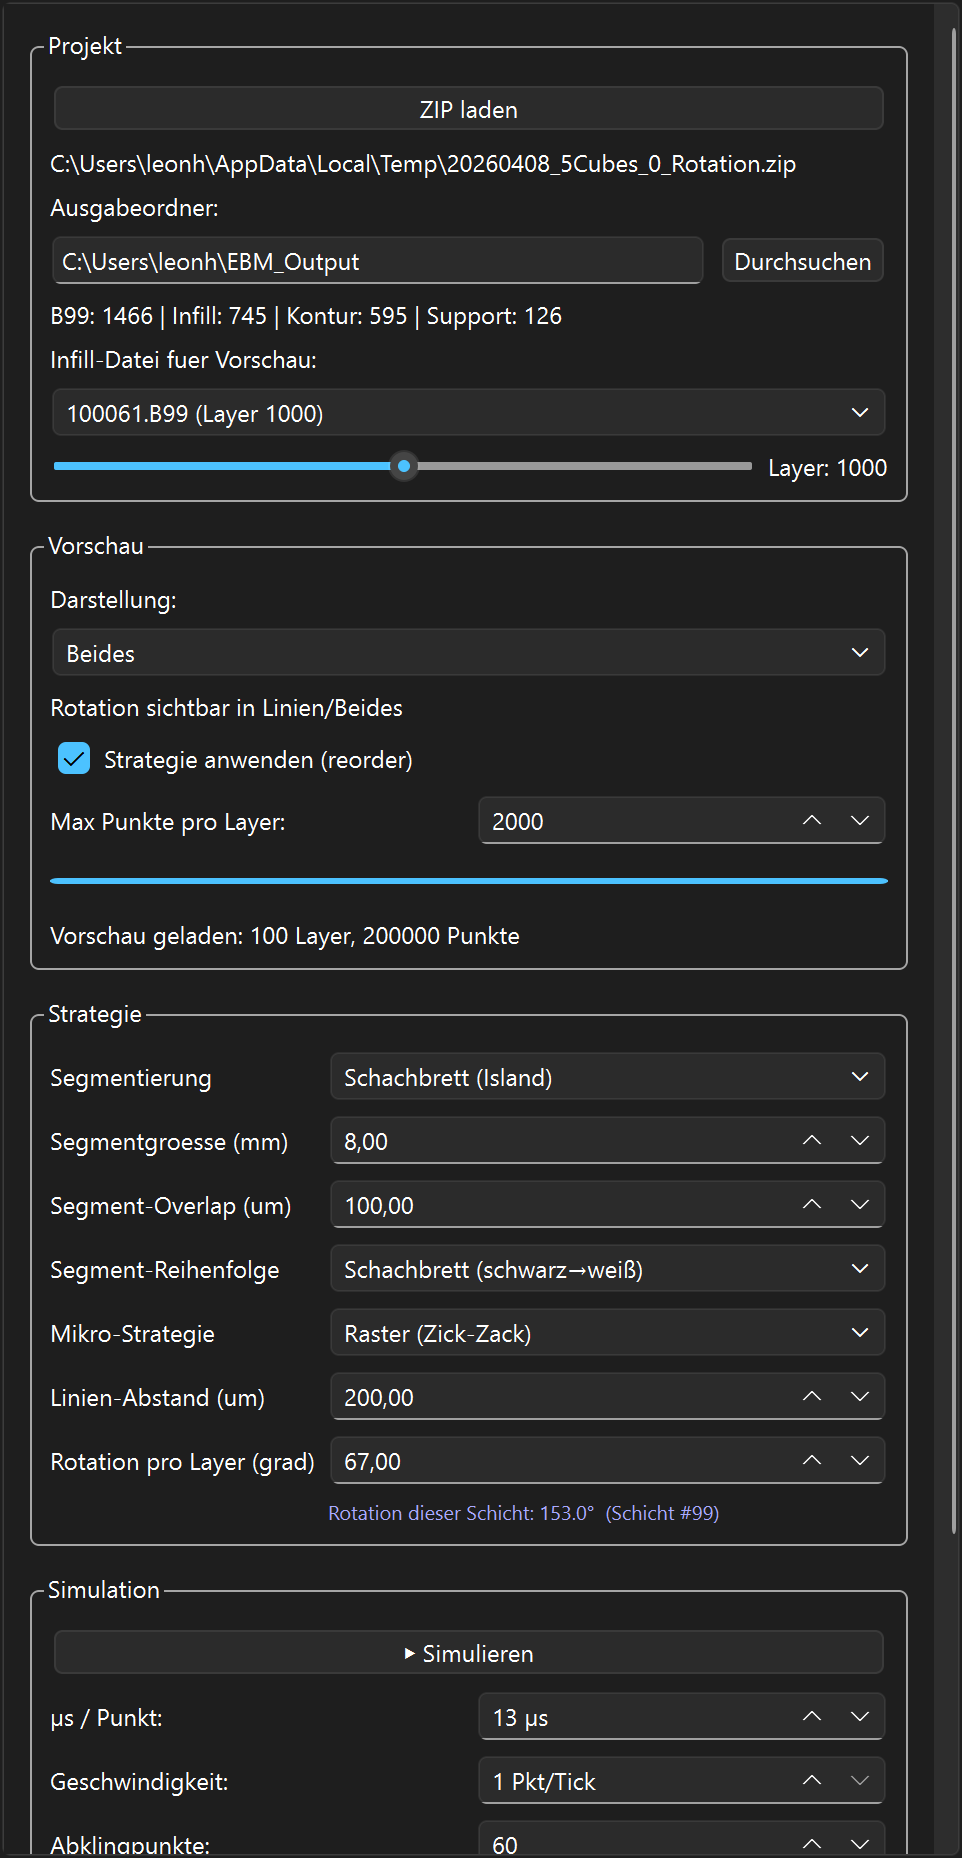
\includegraphics[height=0.82\textheight]{screenshots/04_bedienpanel.png}
  \caption{Das Bedien-Panel im Detail mit konfigurierter
           Schachbrett-Segmentierung und Raster-Mikrostrategie. Unter dem
           Rotationsfeld wird die effektive Rotation der aktuellen Schicht
           angezeigt.}
  \label{fig:ebm-panel}
\end{figure}

% ---------------------------------------------------------------------
\subsection{Schritt 3 -- Vorschau und Simulation prüfen}
\label{subsec:ebm-preview}

Im Bereich \emph{Vorschau} steuert das Feld \textbf{Darstellung} die Ansicht:
\emph{Punkte} zeigt nur die Schmelzpunkte, \emph{Linien} den Scan-Pfad und
\emph{Beides} die Kombination. Mit dem Schieberegler \emph{Layer} lässt sich
durch die Schichten blättern; jede Änderung an der Strategie aktualisiert die
Vorschau automatisch. Abbildung~\ref{fig:ebm-strategy} zeigt die
Schachbrett-Strategie über mehrere übereinanderliegende Schichten, wodurch die
schichtweise Rotation sichtbar wird.

\begin{figure}[H]
  \centering
  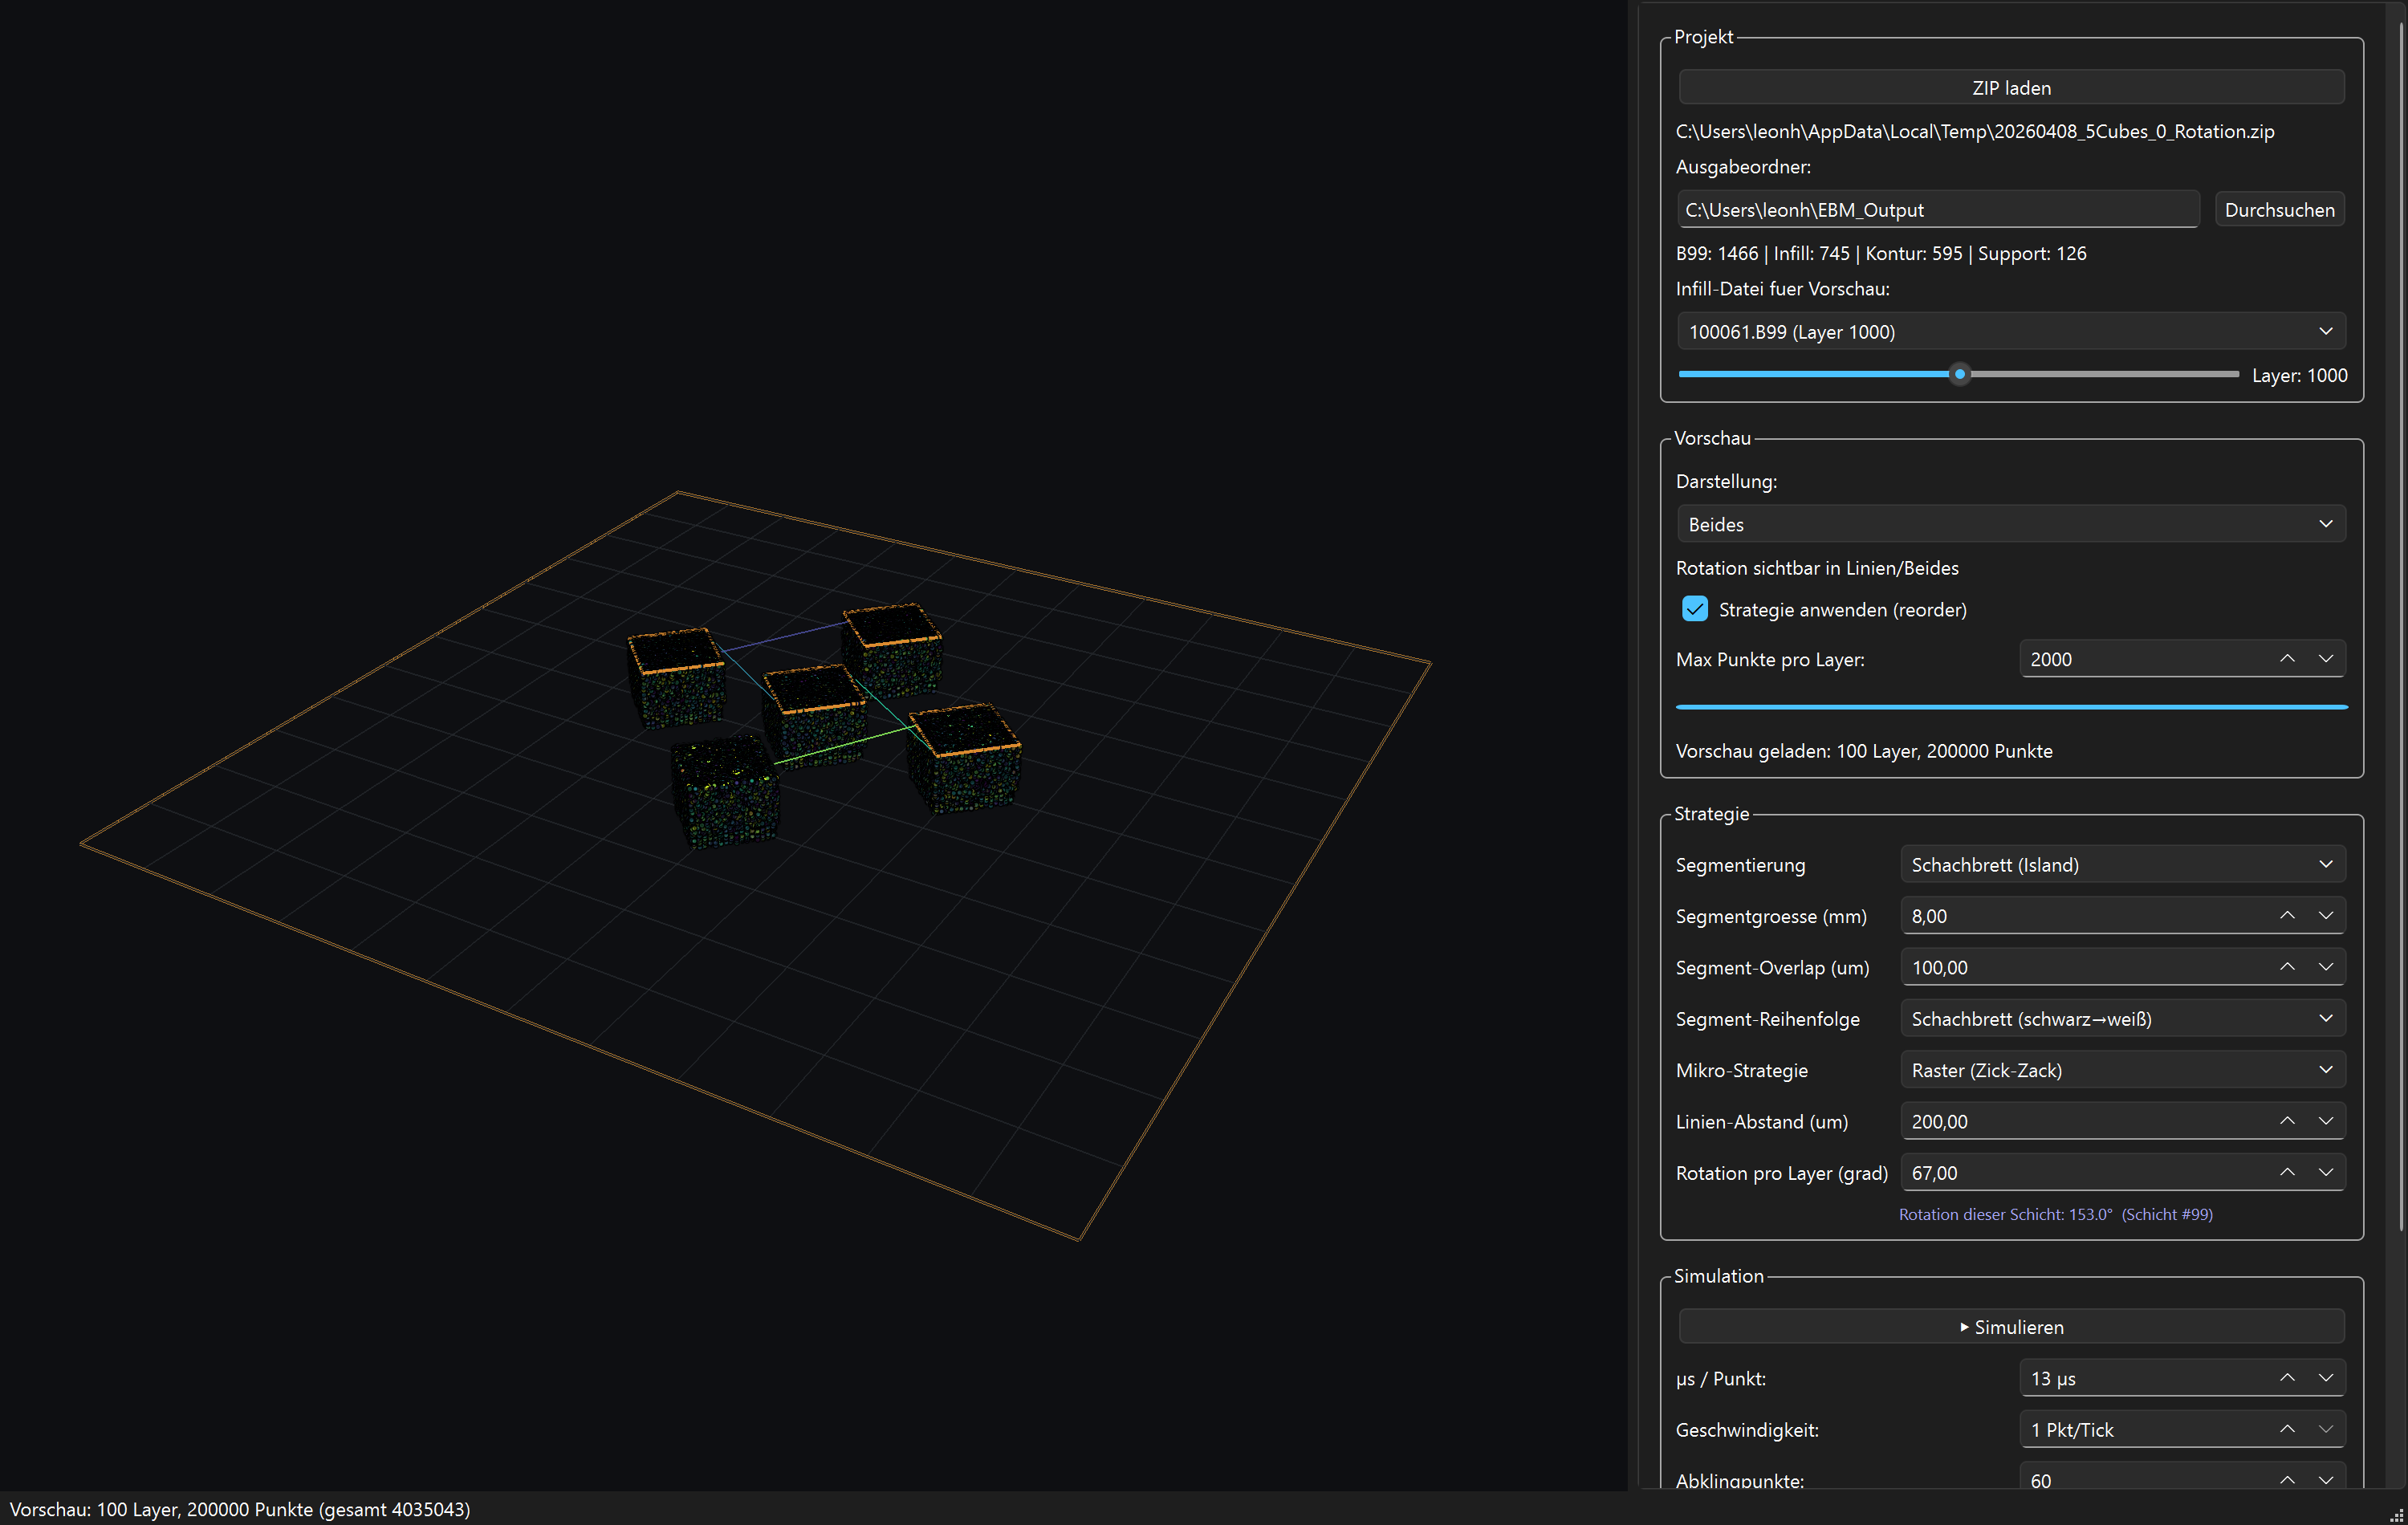
\includegraphics[width=\linewidth]{screenshots/03_strategie_vorschau.png}
  \caption{3D-Vorschau mit aktiver Schachbrett-Segmentierung und
           schichtweiser Rotation. Die grünen Linien zeigen den Scan-Pfad der
           aktuell gewählten Schicht.}
  \label{fig:ebm-strategy}
\end{figure}

\paragraph{Simulation.}
Über \textbf{$\blacktriangleright$~Simulieren} im Bereich \emph{Simulation}
wird die Belichtung der gewählten Schicht Punkt für Punkt animiert. Der gerade
belichtete Punkt leuchtet hell auf, bereits belichtete Punkte klingen langsam
ab -- so wird die Reihenfolge der Strategie unmittelbar nachvollziehbar
(Abbildung~\ref{fig:ebm-sim}). Die Parameter steuern das Tempo:

\begin{itemize}
  \item \textbf{$\mu$s / Punkt} -- realistische Haltezeit pro Punkt
        (typisch 13\,$\mu$s).
  \item \textbf{Geschwindigkeit (Pkt/Tick)} -- wie viele Punkte pro Animations-
        schritt gezeichnet werden; höhere Werte beschleunigen den Durchlauf.
  \item \textbf{Abklingpunkte} -- Länge der nachleuchtenden Spur.
\end{itemize}

\begin{figure}[H]
  \centering
  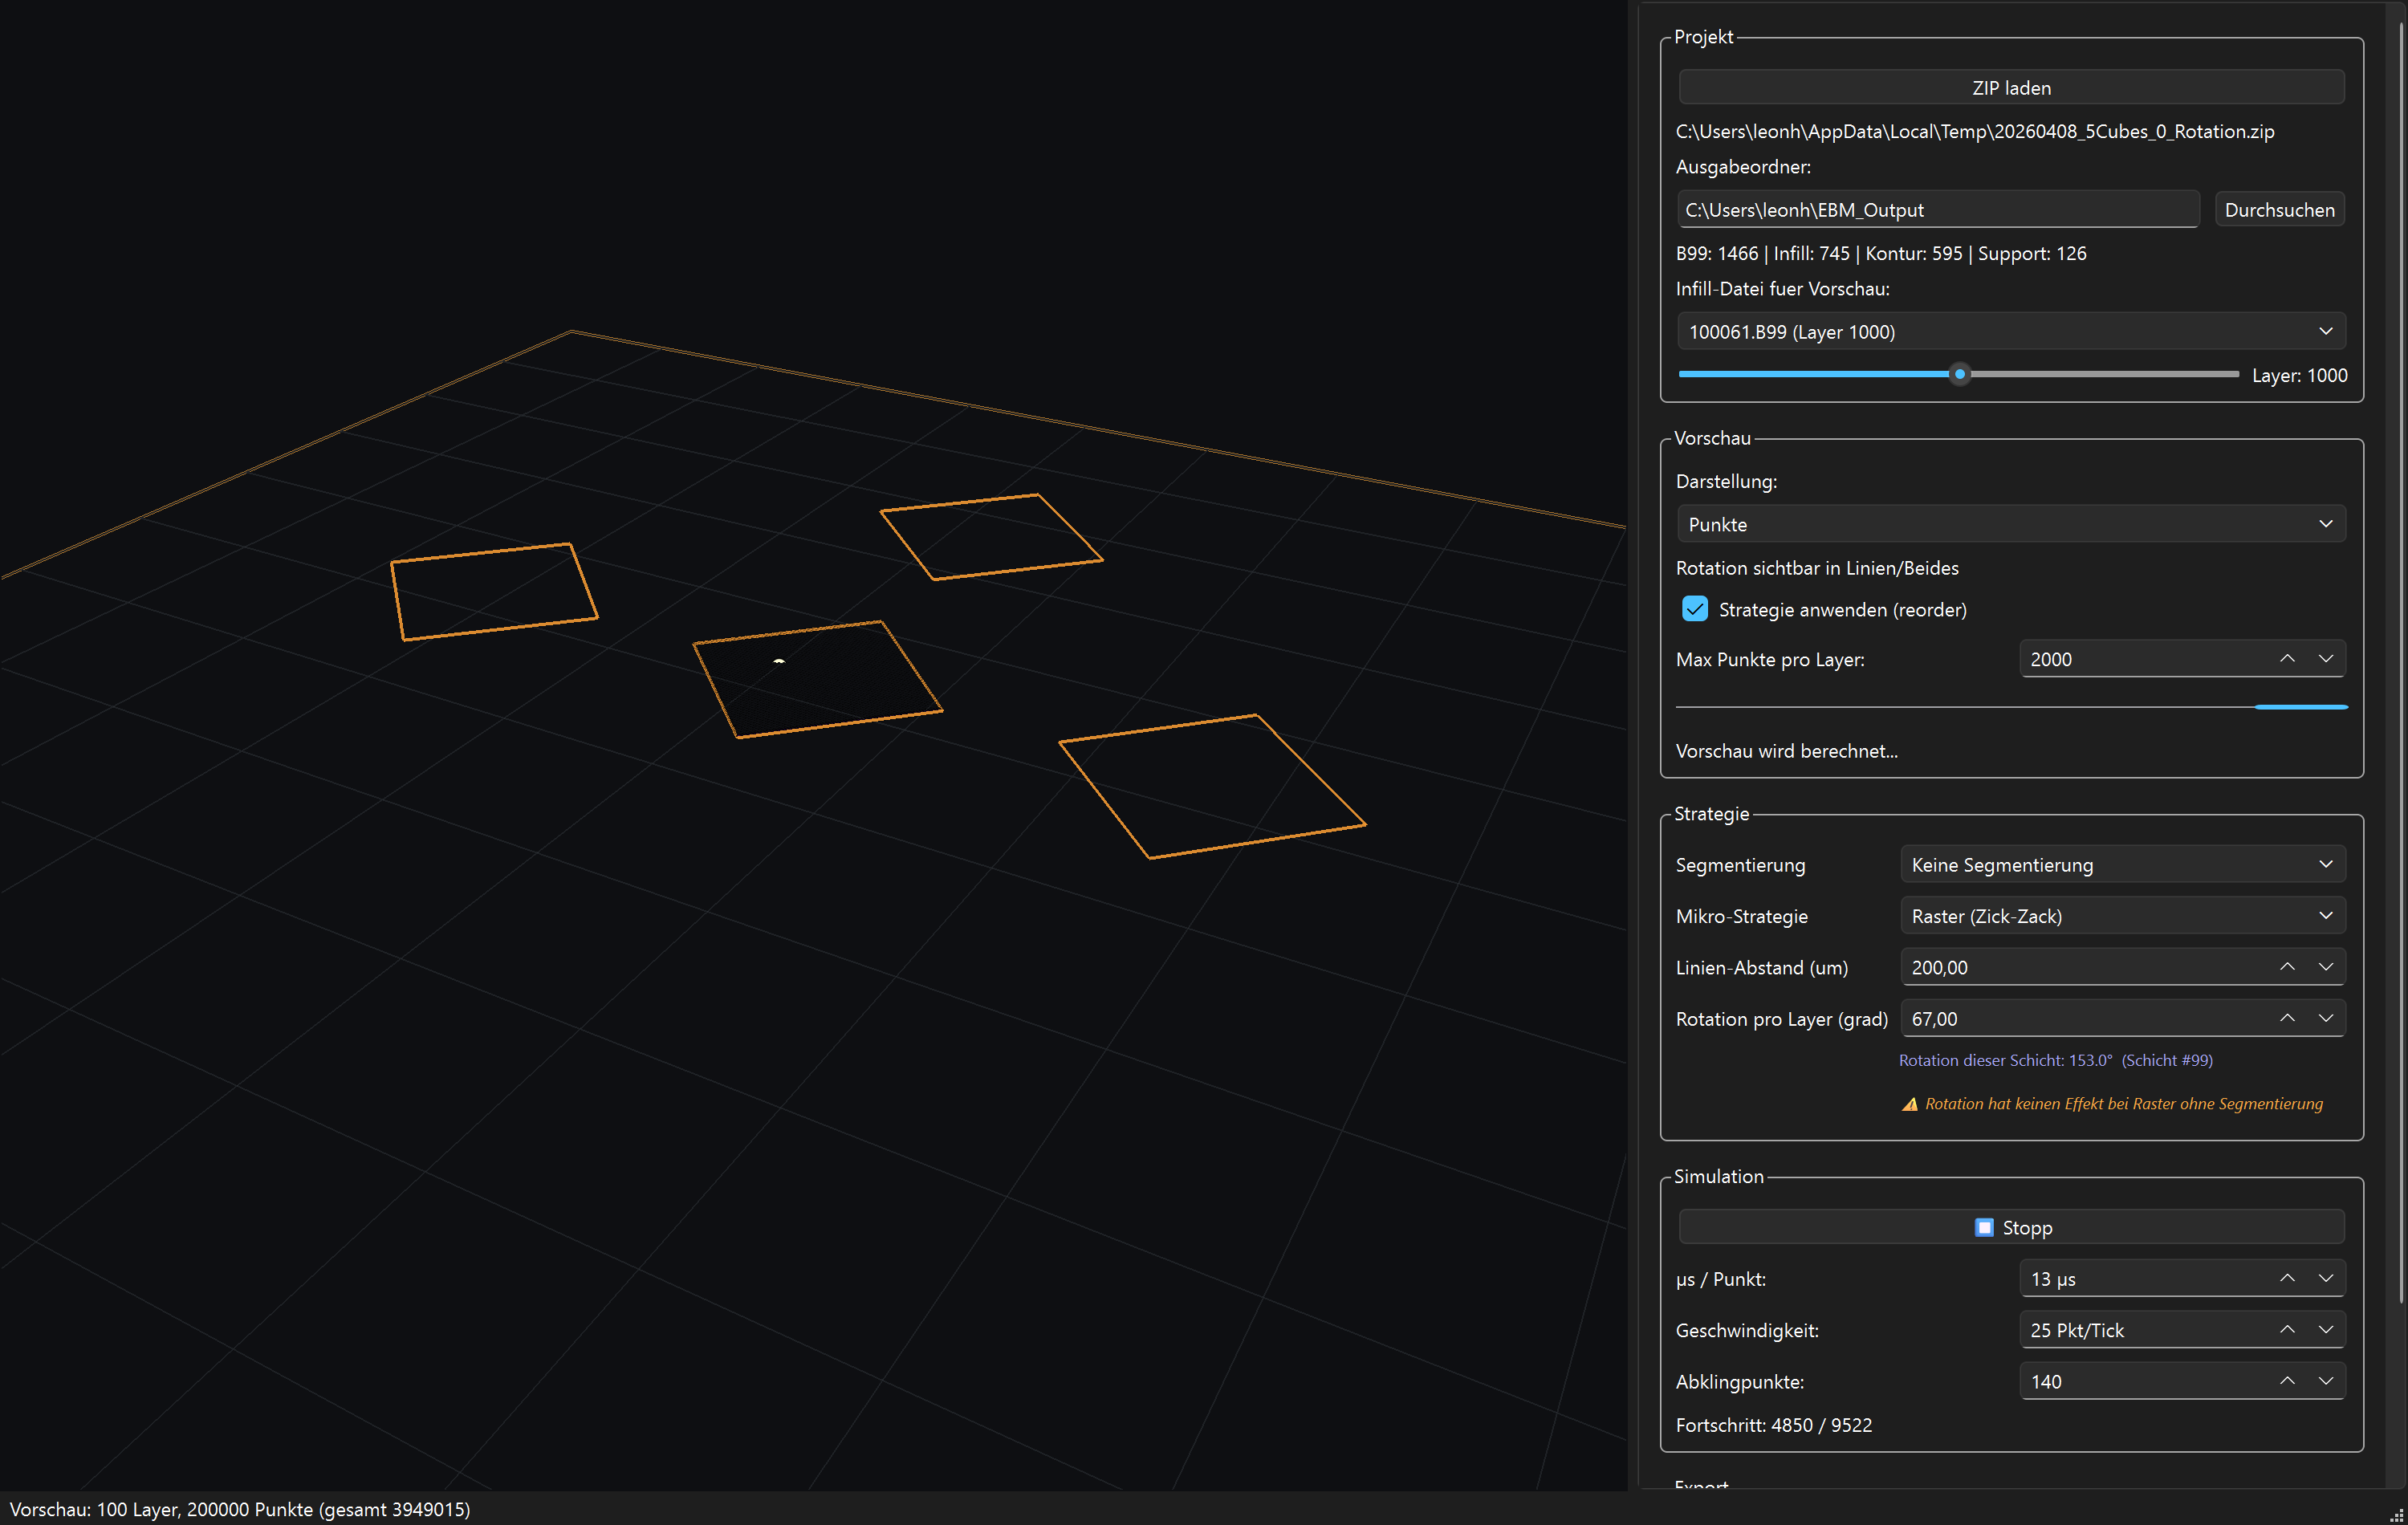
\includegraphics[width=\linewidth]{screenshots/05_simulation.png}
  \caption{Laufende Simulation (herangezoomt). Der helle Punkt markiert die
           aktuelle Strahlposition; die Fortschrittsanzeige zeigt
           \texttt{4850 / 9522}. Über dieselbe Schaltfläche (jetzt
           \texttt{$\blacksquare$ Stopp}) wird die Animation beendet.}
  \label{fig:ebm-sim}
\end{figure}

% ---------------------------------------------------------------------
\subsection{Schritt 4 -- Druckfertiges ZIP exportieren}
\label{subsec:ebm-export}

Ist die Strategie eingestellt, erzeugt die Schaltfläche \textbf{Strategie
anwenden \& ZIP erstellen} im Bereich \emph{Export} das fertige Archiv. Die
Software wendet die gewählte Strategie auf \emph{alle} Infill-Schichten an
(Kontur- und Stützstrukturdateien bleiben unverändert) und legt das Ergebnis
als \texttt{<name>\_NEW.zip} im konfigurierten Ausgabeordner ab. Ein
Fortschrittsbalken zeigt den Verlauf, nach Abschluss erscheint der vollständige
Pfad der erzeugten Datei.

\begin{quote}
  \footnotesize
  Die ursprünglich extrahierten Dateien werden dabei nie verändert. Jeder
  Export arbeitet auf einer frischen Kopie -- ein wiederholter Export liefert
  daher stets dasselbe Ergebnis und es kommt zu keiner doppelten Umsortierung.
\end{quote}

% ---------------------------------------------------------------------
\subsection{Zusammenfassung des Arbeitsablaufs}
\label{subsec:ebm-summary}

\begin{enumerate}
  \item \textbf{ZIP laden} -- Baujob-Archiv mit \texttt{Figure Files/} öffnen.
  \item \textbf{Strategie wählen} -- Segmentierung, Mikro-Strategie und
        Rotation pro Schicht einstellen.
  \item \textbf{Vorschau / Simulation} -- Ergebnis in der 3D-Ansicht prüfen.
  \item \textbf{Export} -- druckfertiges \texttt{*\_NEW.zip} erzeugen.
\end{enumerate}


\end{document}
